% !TEX program = xelatex
% !TEX encoding = UTF-8 Unicode
\documentclass[aspectratio=169]{beamer}
\usetheme{default}
\usefonttheme{professionalfonts}

\usepackage[T1]{fontenc}
\usepackage{lmodern}
\usepackage{graphicx}
\usepackage{booktabs}
\usepackage{amsmath}
\usepackage{array}
\usepackage{xcolor}

\definecolor{PrimaryBlue}{HTML}{0F4C81}
\definecolor{PrimaryBlueDark}{HTML}{0B395F}
\definecolor{AccentTeal}{HTML}{127C8A}
\definecolor{BodyText}{HTML}{1F2937}
\definecolor{MutedText}{HTML}{6B7280}
\definecolor{SoftPanel}{HTML}{F4F7FB}

\setbeamercolor{normal text}{fg=BodyText,bg=white}
\setbeamercolor{structure}{fg=PrimaryBlue}
\setbeamercolor{frametitle}{fg=white,bg=PrimaryBlue}
\setbeamercolor{title}{fg=white,bg=PrimaryBlue}
\setbeamercolor{subtitle}{fg=white,bg=PrimaryBlue}
\setbeamercolor{section in toc}{fg=PrimaryBlueDark}
\setbeamercolor{subsection in toc}{fg=BodyText}
\setbeamercolor{author in head/foot}{fg=white,bg=PrimaryBlueDark}
\setbeamercolor{date in head/foot}{fg=white,bg=AccentTeal}
\setbeamercolor{block title}{fg=white,bg=PrimaryBlue}
\setbeamercolor{block body}{fg=BodyText,bg=SoftPanel}
\setbeamercolor{itemize item}{fg=AccentTeal}
\setbeamercolor{itemize subitem}{fg=PrimaryBlue}
\setbeamerfont{title}{size=\LARGE,series=\bfseries}
\setbeamerfont{subtitle}{size=\large}
\setbeamerfont{frametitle}{size=\large,series=\bfseries}
\setbeamerfont{footline}{size=\scriptsize}

\setbeamertemplate{navigation symbols}{}
\setbeamertemplate{blocks}[rounded][shadow=false]
\setbeamertemplate{itemize item}{\color{AccentTeal}\large$\bullet$}
\setbeamertemplate{itemize subitem}{\color{PrimaryBlue}$\triangleright$}

\setbeamertemplate{frametitle}{
  \nointerlineskip
  \begin{beamercolorbox}[
    wd=\paperwidth,
    ht=3.4ex,
    dp=1.15ex,
    leftskip=1.2em,
    rightskip=0.8em
  ]{frametitle}
    \usebeamerfont{frametitle}\insertframetitle
  \end{beamercolorbox}
}

\setbeamertemplate{footline}{
  \leavevmode
  \hbox{
    \begin{beamercolorbox}[wd=.82\paperwidth,ht=2.8ex,dp=1.15ex,leftskip=1.1em]{author in head/foot}
      \usebeamerfont{footline}\insertshorttitle
    \end{beamercolorbox}
    \begin{beamercolorbox}[wd=.18\paperwidth,ht=2.8ex,dp=1.15ex,rightskip=1.0em plus1fil]{date in head/foot}
      \usebeamerfont{footline}\insertframenumber/\inserttotalframenumber
    \end{beamercolorbox}
  }
}

\graphicspath{{assets/generated/}}

\title[Image\_projet\_money]{Image\_projet\_money \\ Coin Detection and Value Estimation}
\subtitle{Master 1 -- VMI Analyse d'Image}
\author{Maksym Dolhov, Mehdi Aghaei, Nima Davari}
\institute{Universite Paris Cite}
\date{\today}

\begin{document}

\begin{frame}
  \titlepage
  \vspace{-0.4em}
  \centering
  \small \textbf{GitHub: }
  \href{https://github.com/sorooshaghaei/Image_projet_money}{\texttt{github.com/sorooshaghaei/Image\_projet\_money}}
\end{frame}

\begin{frame}{Presentation Plan (15 minutes)}
  \tableofcontents
\end{frame}

\section{Problem and Data}

\begin{frame}{Project Goal}
  \begin{itemize}
    \item Input: one RGB image with multiple euro coins on different surfaces and lighting conditions.
    \item Output 1: number of detected coins.
    \item Output 2: estimated total value (in EUR/cents).
    \item Constraint: use classical computer vision + deterministic heuristics from our implemented codebase.
    \item Main code references: \texttt{main.py}, \texttt{src/}, \texttt{PIPELINE.md}, \texttt{README.md}.
  \end{itemize}
\end{frame}

\begin{frame}{Dataset and Evaluation Protocol}
  \begin{itemize}
    \item Dataset folder: \texttt{data/images/} with groups \texttt{gp1} ... \texttt{gp8}.
    \item Ground truth source: \texttt{src/data/ground\_truth.py} (\texttt{RAW\_ANNOTATIONS} table).
    \item Processed images: 106.
    \item Evaluated with ground truth: 105 (1 image skipped: missing value/annotation row).
    \item Metrics computed by \texttt{src/evaluation/metrics.py}; report rows written by \texttt{src/evaluation/reporting.py}.
  \end{itemize}

  \vspace{0.3em}
  \begin{tabular}{@{}ll@{}}
    \toprule
    Metric (current run) & Value \\
    \midrule
    Coin exact-match accuracy & 76.19\% (80/105) \\
    Value evaluated images & 103/105 \\
    Value MAE & 1.791 EUR per image \\
    Value MSE & 15.3455 EUR\(^2\) per image \\
    \bottomrule
  \end{tabular}
\end{frame}

\section{Implemented Methods}

\begin{frame}{End-to-End Method Flow}
  \centering
  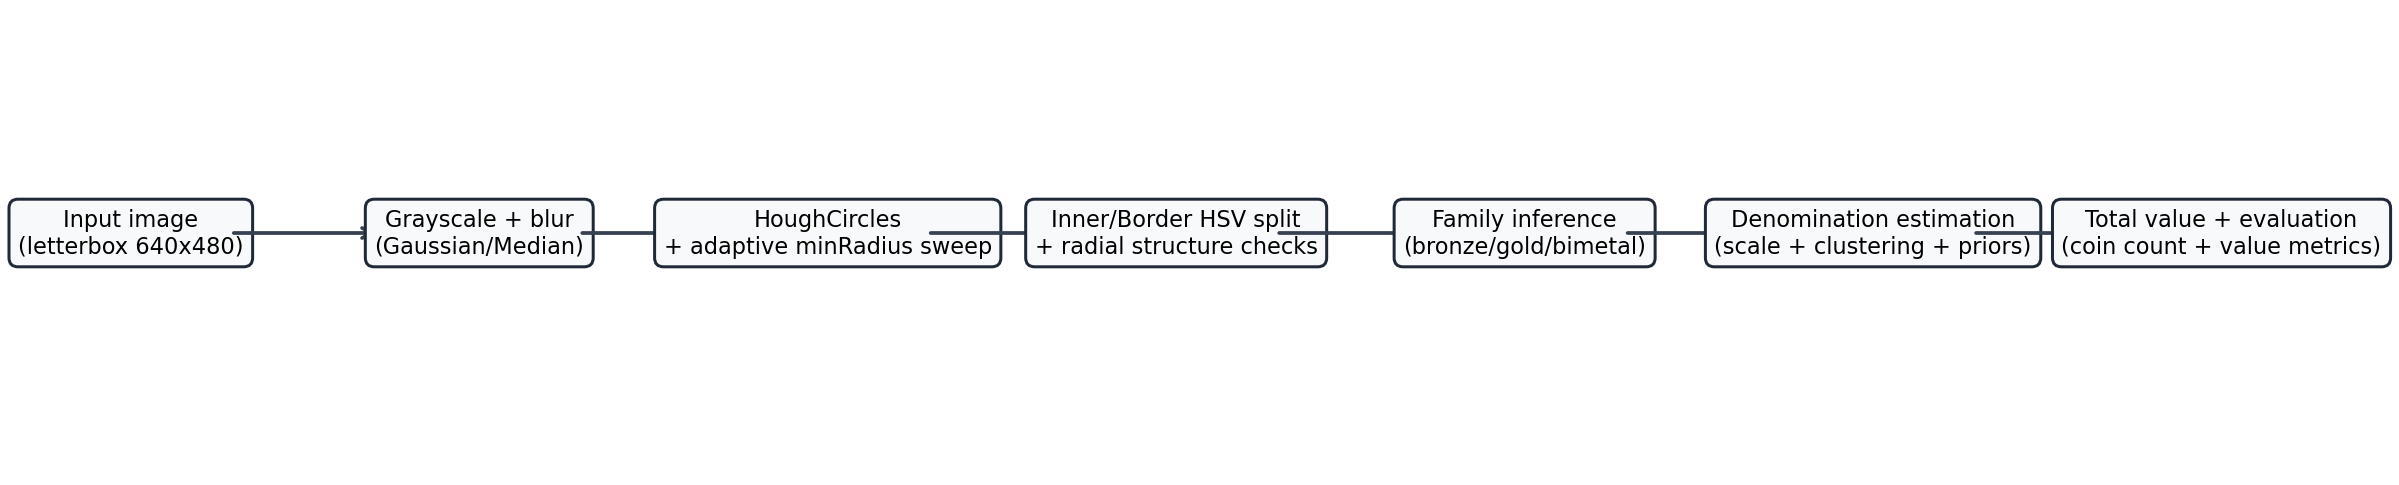
\includegraphics[width=\linewidth]{methods_flow.png}
\end{frame}

\begin{frame}{How We Read Data (Code-backed)}
  \begin{itemize}
    \item \texttt{ImageDataset.list\_images()} recursively scans \texttt{data/images/} and keeps only valid extensions
    (\texttt{src/data/dataset.py}).
    \item Files are sorted by relative path so runs are deterministic and reproducible.
    \item Group aliases are normalized (\texttt{grp3} \(\rightarrow\) \texttt{gp3}) before matching
    (\texttt{normalize\_group\_name}).
    \item \texttt{GroundTruthRepository} parses \texttt{RAW\_ANNOTATIONS} and supports comma/dot decimals
    (\texttt{src/data/ground\_truth.py}).
    \item CLI matches each image with GT by \((group, filename)\); missing GT is marked \texttt{SKIP\_NO\_GT}
    (\texttt{src/app/cli.py}).
  \end{itemize}
\end{frame}

\begin{frame}{Preprocessing Choices and Why}
  \begin{tabular}{@{}p{0.36\linewidth}p{0.58\linewidth}@{}}
    \toprule
    Step (implemented) & Reason in our pipeline \\
    \midrule
    Letterbox to \(640 \times 480\) & Keep geometric scale consistent so Hough thresholds and radius sweeps are comparable across mixed image resolutions. \\
    RGB \(\rightarrow\) grayscale & Reduce color variability; keep intensity/edge information needed by Hough circles. \\
    Gaussian or median blur & Suppress high-frequency texture noise before circle voting; reduce false circles from background patterns. \\
    Auto \texttt{param1} from Scharr gradient percentile & Scene-adaptive Canny thresholding inside Hough; avoids brittle fixed-edge threshold on easy vs hard backgrounds. \\
    Runtime normalization path & Current implementation keeps preprocessing compact: grayscale + blur for stable cross-group behavior. \\
    \bottomrule
  \end{tabular}
\end{frame}

\begin{frame}{Processing and Model Choices: Why These Methods}
  \begin{tabular}{@{}p{0.34\linewidth}p{0.60\linewidth}@{}}
    \toprule
    Method & Why we used it \\
    \midrule
    \texttt{cv2.HoughCircles} + adaptive \texttt{minRadius} sweep & Coins are near-circular; sweep + geometry penalties (nested/intrusion checks) makes detection robust when one fixed radius fails. \\
    Inner/Border HSV split + radial structure checks & Bimetal vs single-color requires radial evidence, not only global color. We add KMeans radial separation and radial step checks for this. \\
    Family inference (\texttt{bronze/gold/bimetal}) & Constrains denomination search space early and reduces confusion between visually close coins. \\
    Scale + family-wise radius clustering + priors & Maps pixel radii to denomination probabilities even when camera distance changes; combines size likelihood + cluster priors + center proximity. \\
    Deterministic rules + debug overlays & Gives explainable decisions per coin and supports slide-level diagnostics for failures and successes. \\
    \bottomrule
  \end{tabular}
\end{frame}

\begin{frame}{Stage 1: Preprocessing}
  \begin{itemize}
    \item Letterbox normalization to fixed canvas \(640 \times 480\) (\texttt{letterbox\_resize\_to\_canvas}).
    \item RGB \(\rightarrow\) grayscale conversion.
    \item Blur mode configurable (\texttt{gauss} or \texttt{median}); active default is Gaussian.
    \item Effective detection path uses grayscale + blur.
    \item Objective: stabilize Hough detection across heterogeneous image resolutions/backgrounds.
  \end{itemize}
\end{frame}

\begin{frame}{Stage 2: Circle Detection}
  \begin{itemize}
    \item Core detector: \texttt{cv2.HoughCircles} in \texttt{CoinDetector}.
    \item \texttt{param1} is auto-estimated from Scharr gradient distribution.
    \item \texttt{minRadius} is not fixed:
    \begin{itemize}
      \item sweep candidate range;
      \item score each candidate with geometric penalties:
      \item concentric duplicates, nested circles, intrusions, instability.
    \end{itemize}
    \item Selection policy: plateau/stability voting, with fallback when no clean candidate exists.
    \item Output: detected circles + debug overlays + full sweep diagnostics.
  \end{itemize}
\end{frame}

\begin{frame}{Stage 3: Color Analysis (Inner/Border)}
  \begin{itemize}
    \item For each detected circle, split into:
    \begin{itemize}
      \item inner disk;
      \item border ring.
    \end{itemize}
    \item Compute robust HSV descriptors:
    \begin{itemize}
      \item circular hue average (weighted),
      \item median saturation/value,
      \item hue/saturation/value deltas between inner and border.
    \end{itemize}
    \item Add structure evidence:
    \begin{itemize}
      \item radial 2-cluster KMeans consistency,
      \item radial step-change score,
      \item edge roughness score.
    \end{itemize}
    \item Deterministic decision lattice: \texttt{one-color-like}, \texttt{bi-metal-like}, \texttt{uncertain}.
  \end{itemize}
\end{frame}

\begin{frame}{Stage 4: Denomination and Value Estimation}
  \begin{itemize}
    \item Family inference per coin:
    \begin{itemize}
      \item bronze / gold / bimetal / unknown.
    \end{itemize}
    \item Scale estimation (\(px/mm\)):
    \begin{itemize}
      \item uses bimetal references when available,
      \item fallback consensus voting from all radius hypotheses.
    \end{itemize}
    \item Family-wise radius clustering (1D KMeans + model selection).
    \item Probabilistic score fusion for candidate denominations:
    \begin{itemize}
      \item size likelihood,
      \item cluster mapping prior,
      \item center proximity prior.
    \end{itemize}
    \item Aggregate final denomination counts and total value in cents.
  \end{itemize}
\end{frame}

\section{Process Visual Results}

\begin{frame}{Case 1: gp1/25.png with Accuracy Values}
  \centering
  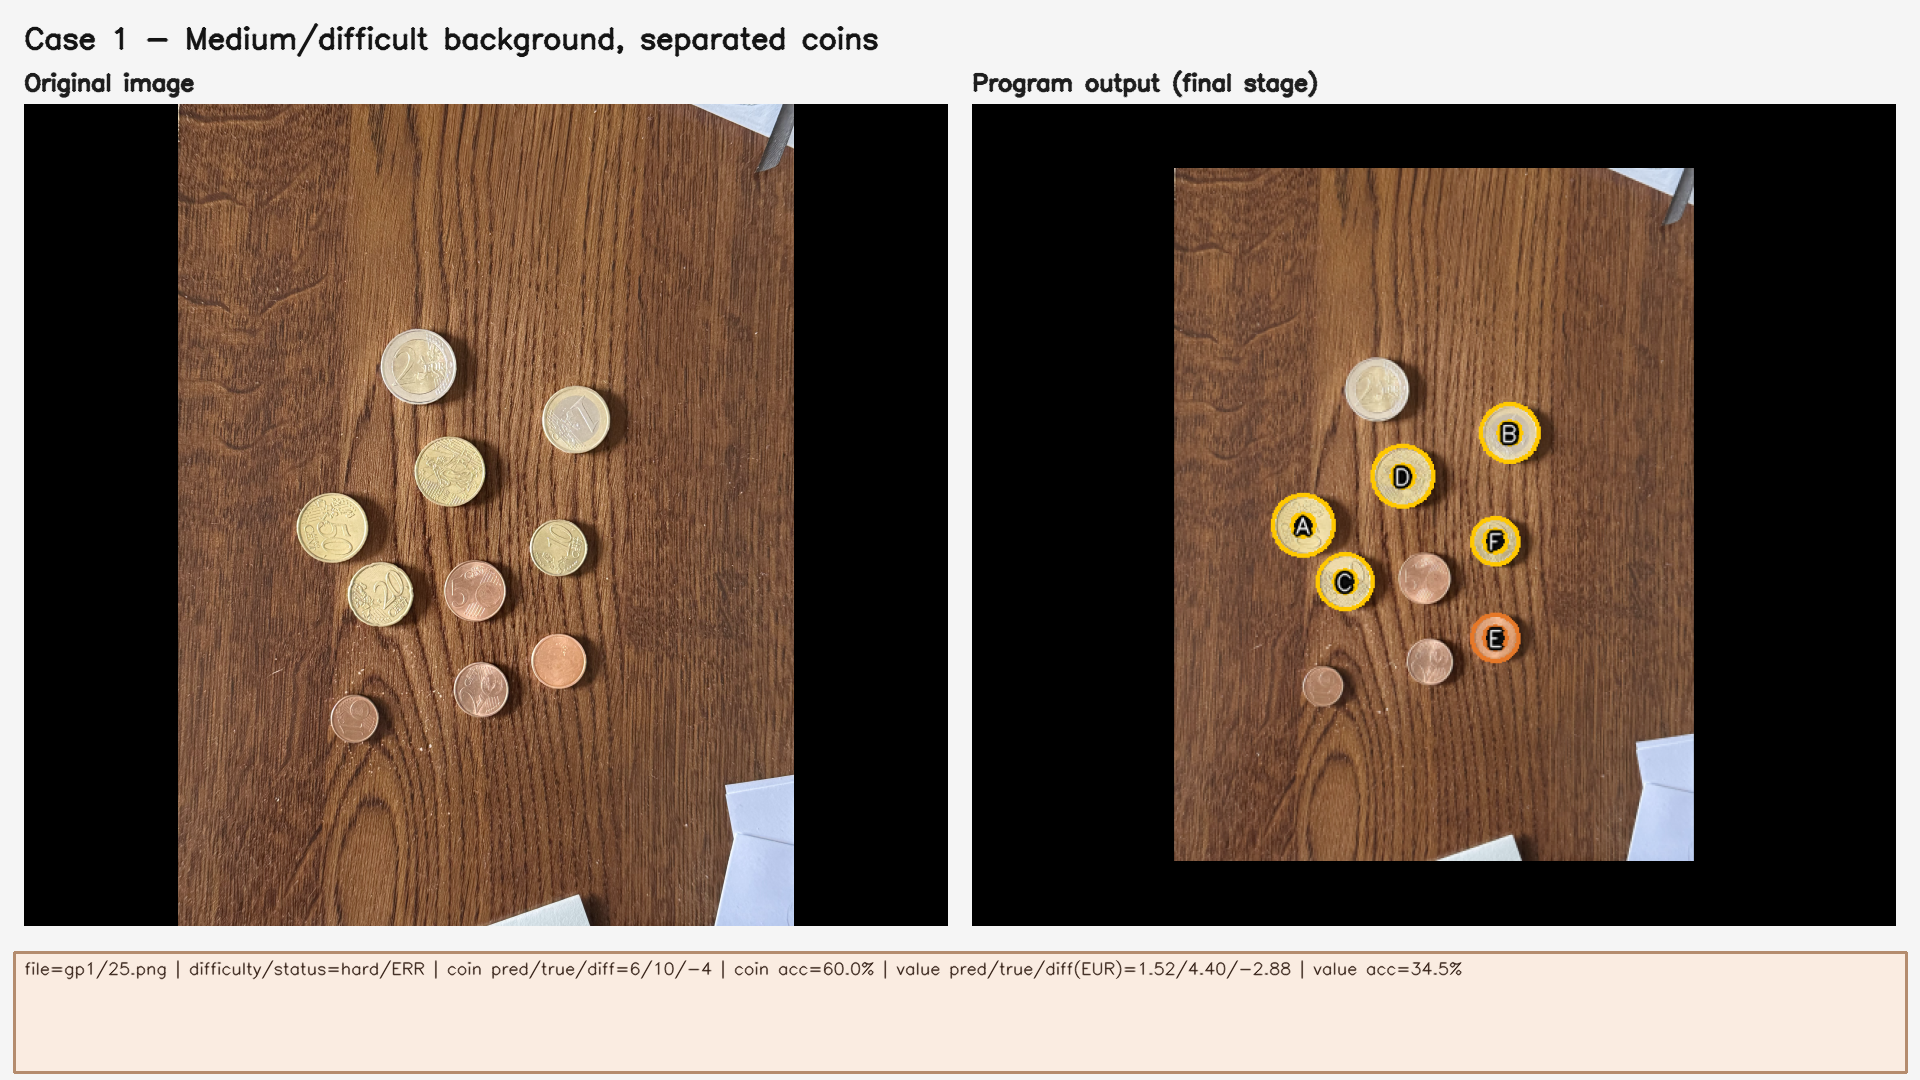
\includegraphics[width=0.985\linewidth,height=0.82\textheight,keepaspectratio]{panel_gp1_25.png}
\end{frame}

\begin{frame}{Case 2: Overlap Coins, Successful Detection/Value}
  \centering
  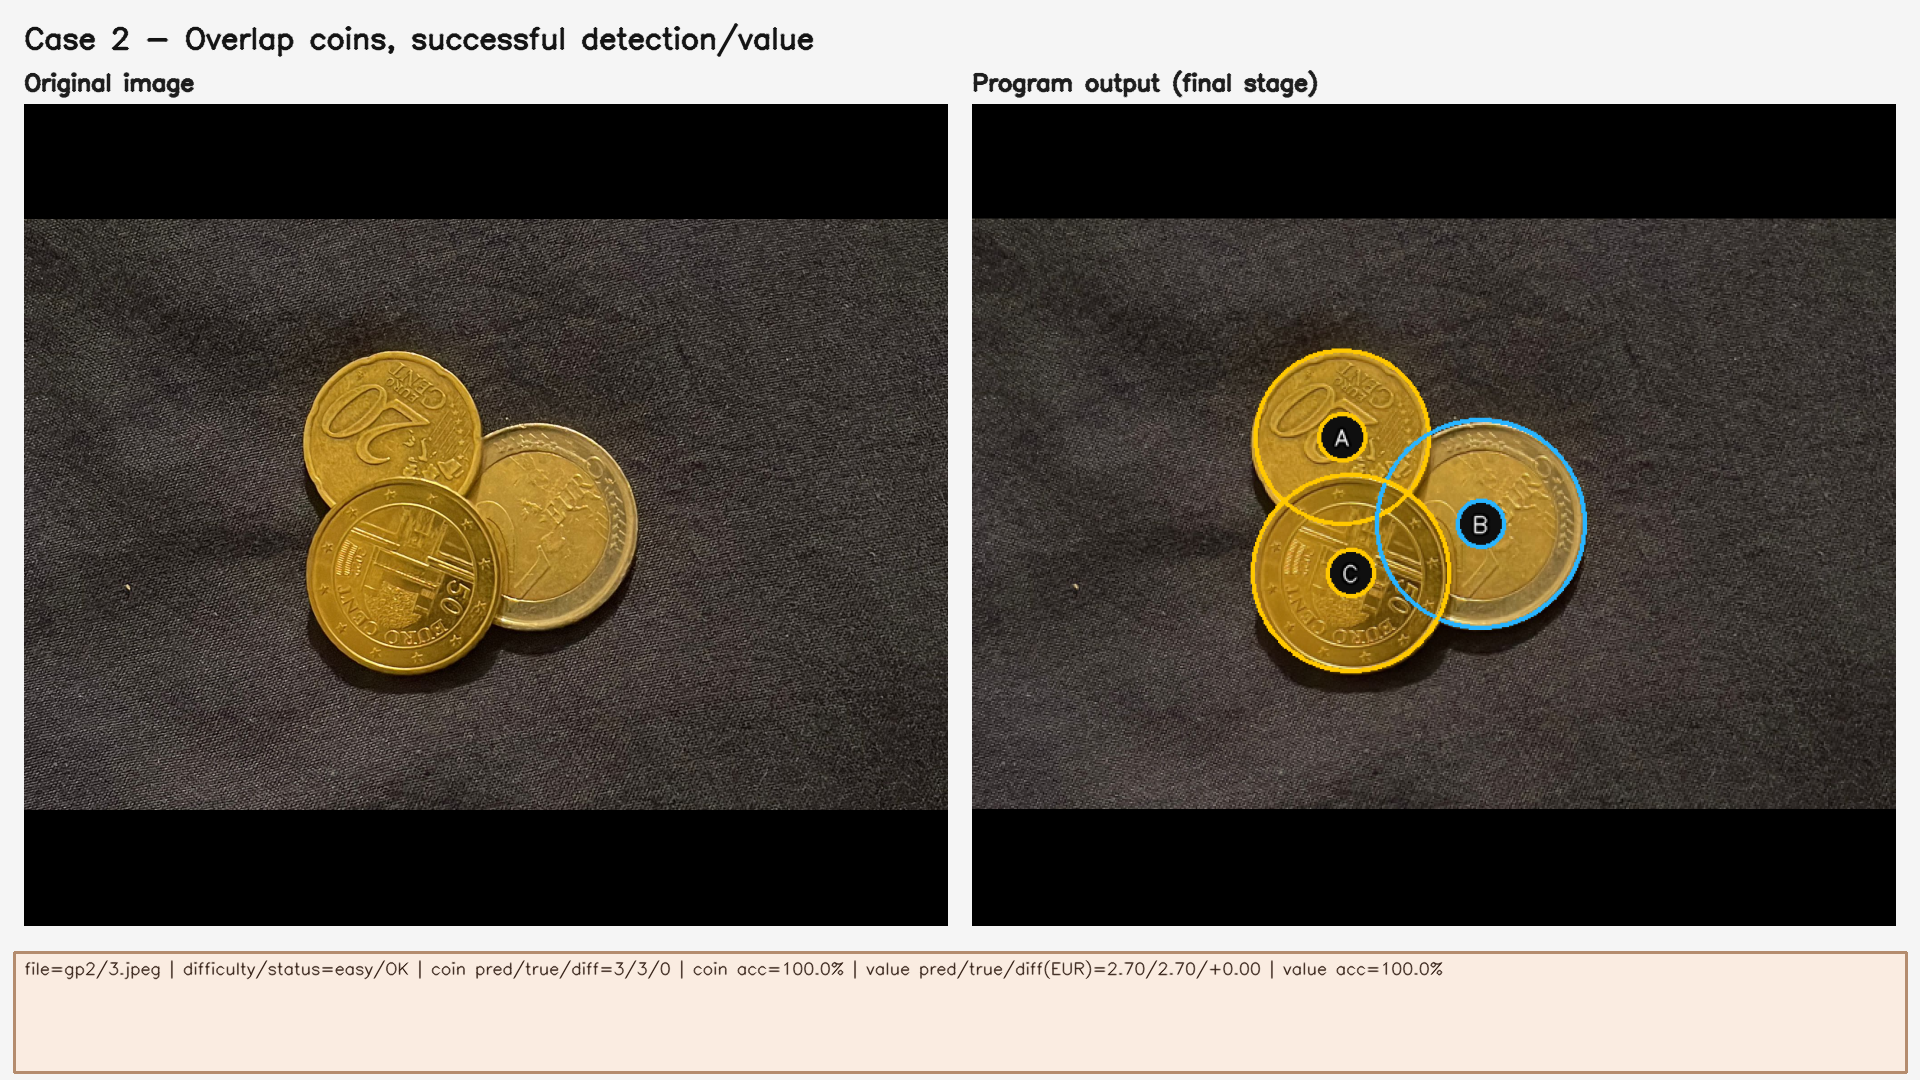
\includegraphics[width=0.985\linewidth,height=0.82\textheight,keepaspectratio]{panel_gp2_3.png}
\end{frame}

\begin{frame}{Case 3: Angle + Reflections (gp3/3\_10.jpg)}
  \centering
  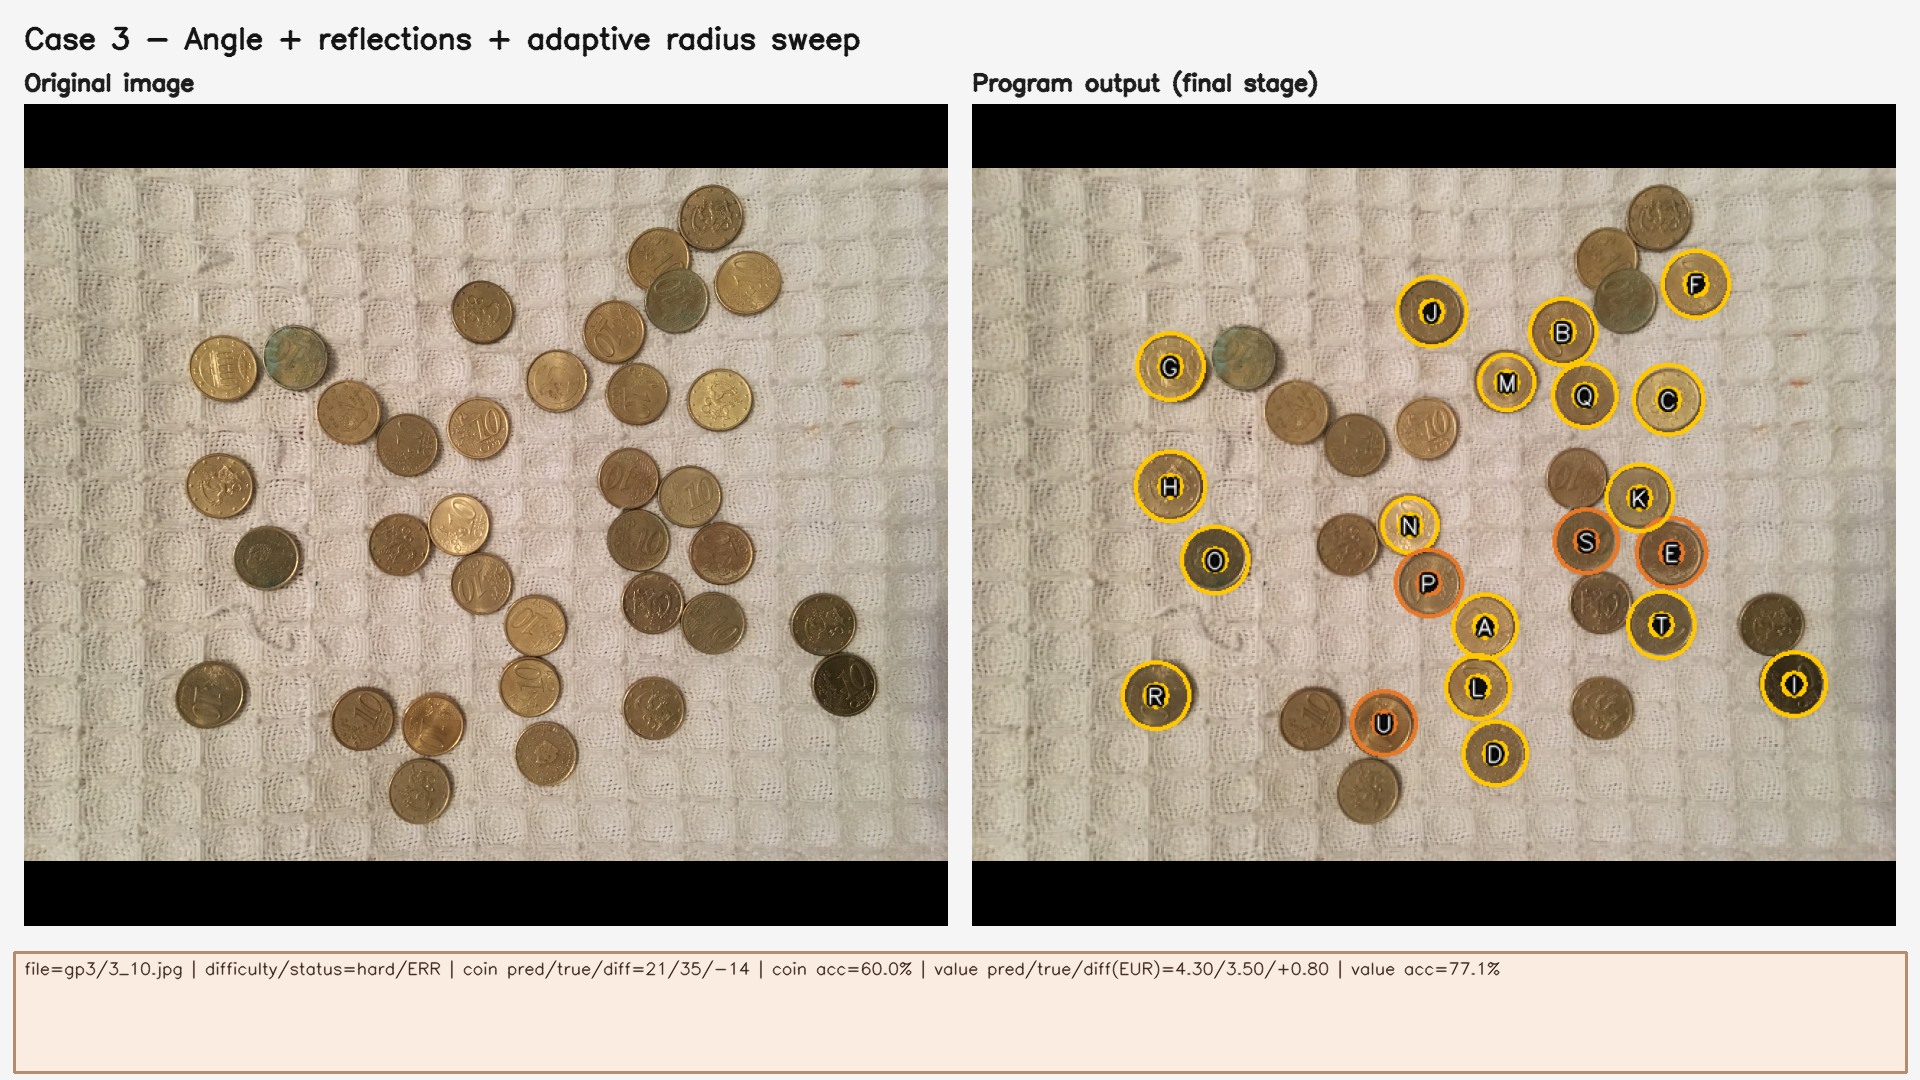
\includegraphics[width=0.985\linewidth,height=0.82\textheight,keepaspectratio]{panel_gp3_3_10.png}
\end{frame}

\begin{frame}{Case 3 Diagnostics: Adaptive Radius Sweep}
  \begin{columns}[T]
    \begin{column}{0.62\textwidth}
      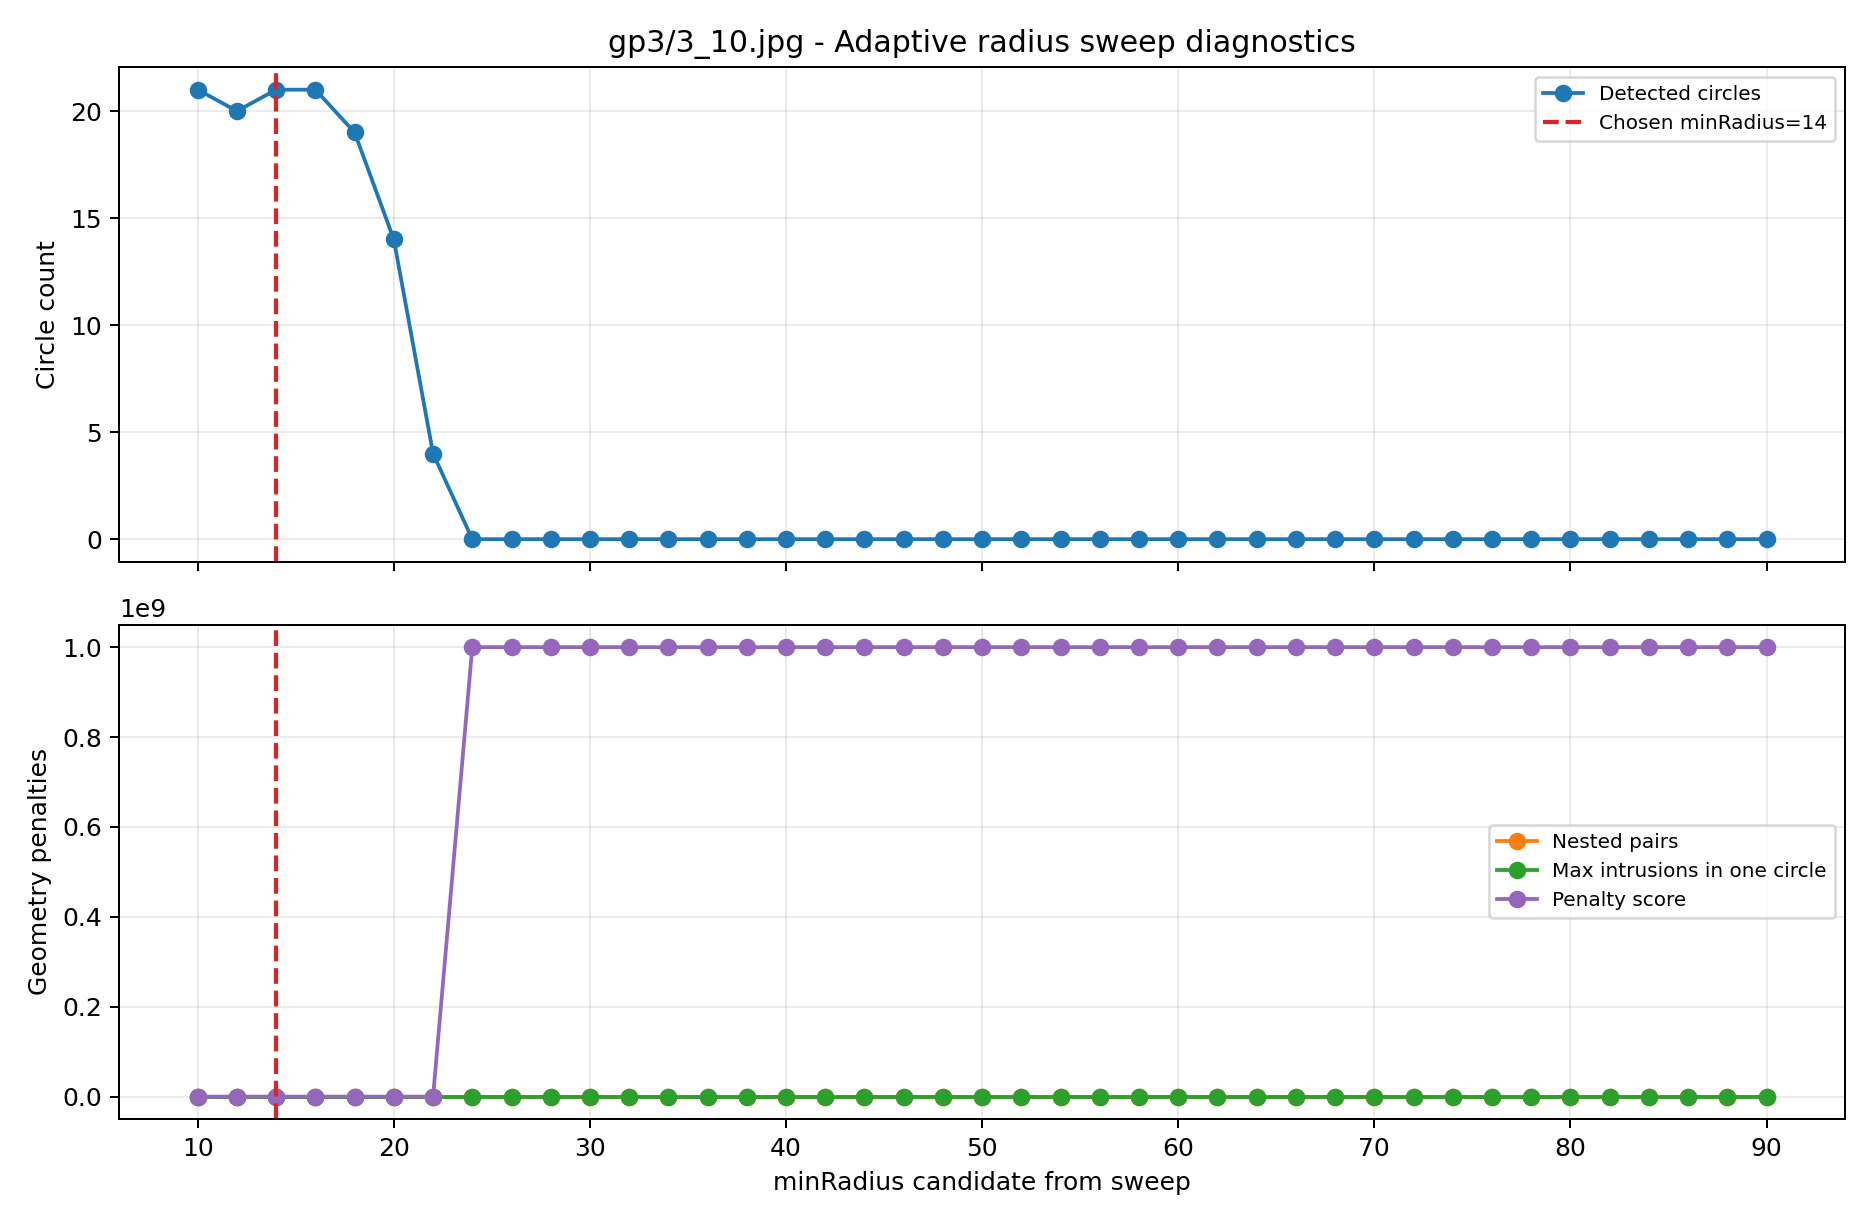
\includegraphics[width=\linewidth]{case_gp3_3_10_sweep_diagnostics.png}
    \end{column}
    \begin{column}{0.38\textwidth}
      \small
      \begin{itemize}
        \item We sweep candidate \texttt{minRadius} values.
        \item Candidates with nested circles or unstable geometry are penalized.
        \item We keep robust plateaus and select the best-supported regime.
        \item This directly addresses angle/reflection sensitivity for \texttt{gp3/3\_10.jpg}.
      \end{itemize}
    \end{column}
  \end{columns}
\end{frame}

\begin{frame}{Case 4A: Difficult Background Close to Coin Color (gp5/0.jpeg)}
  \centering
  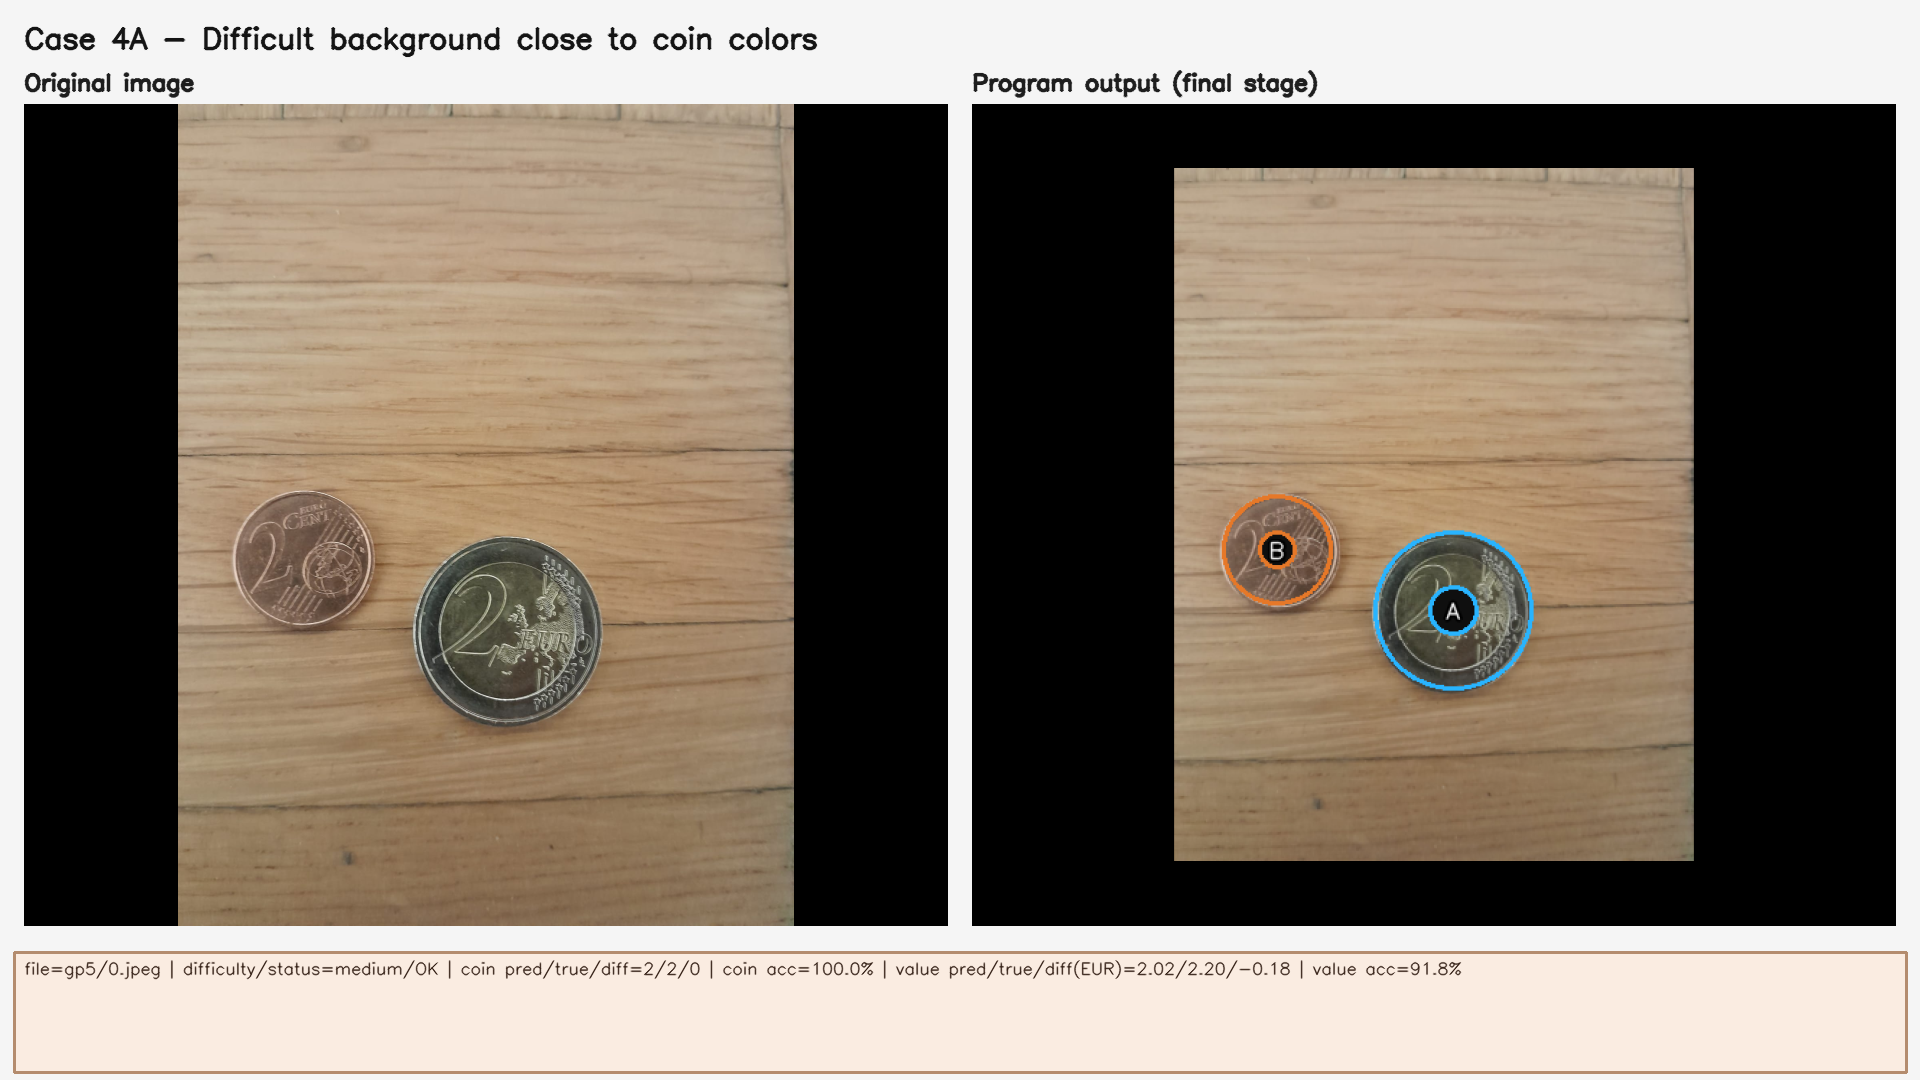
\includegraphics[width=0.985\linewidth,height=0.82\textheight,keepaspectratio]{panel_gp5_0.png}
\end{frame}

\begin{frame}{Case 4B: Difficult Wood Background, Color Confusion (gp5/11.jpg)}
  \centering
  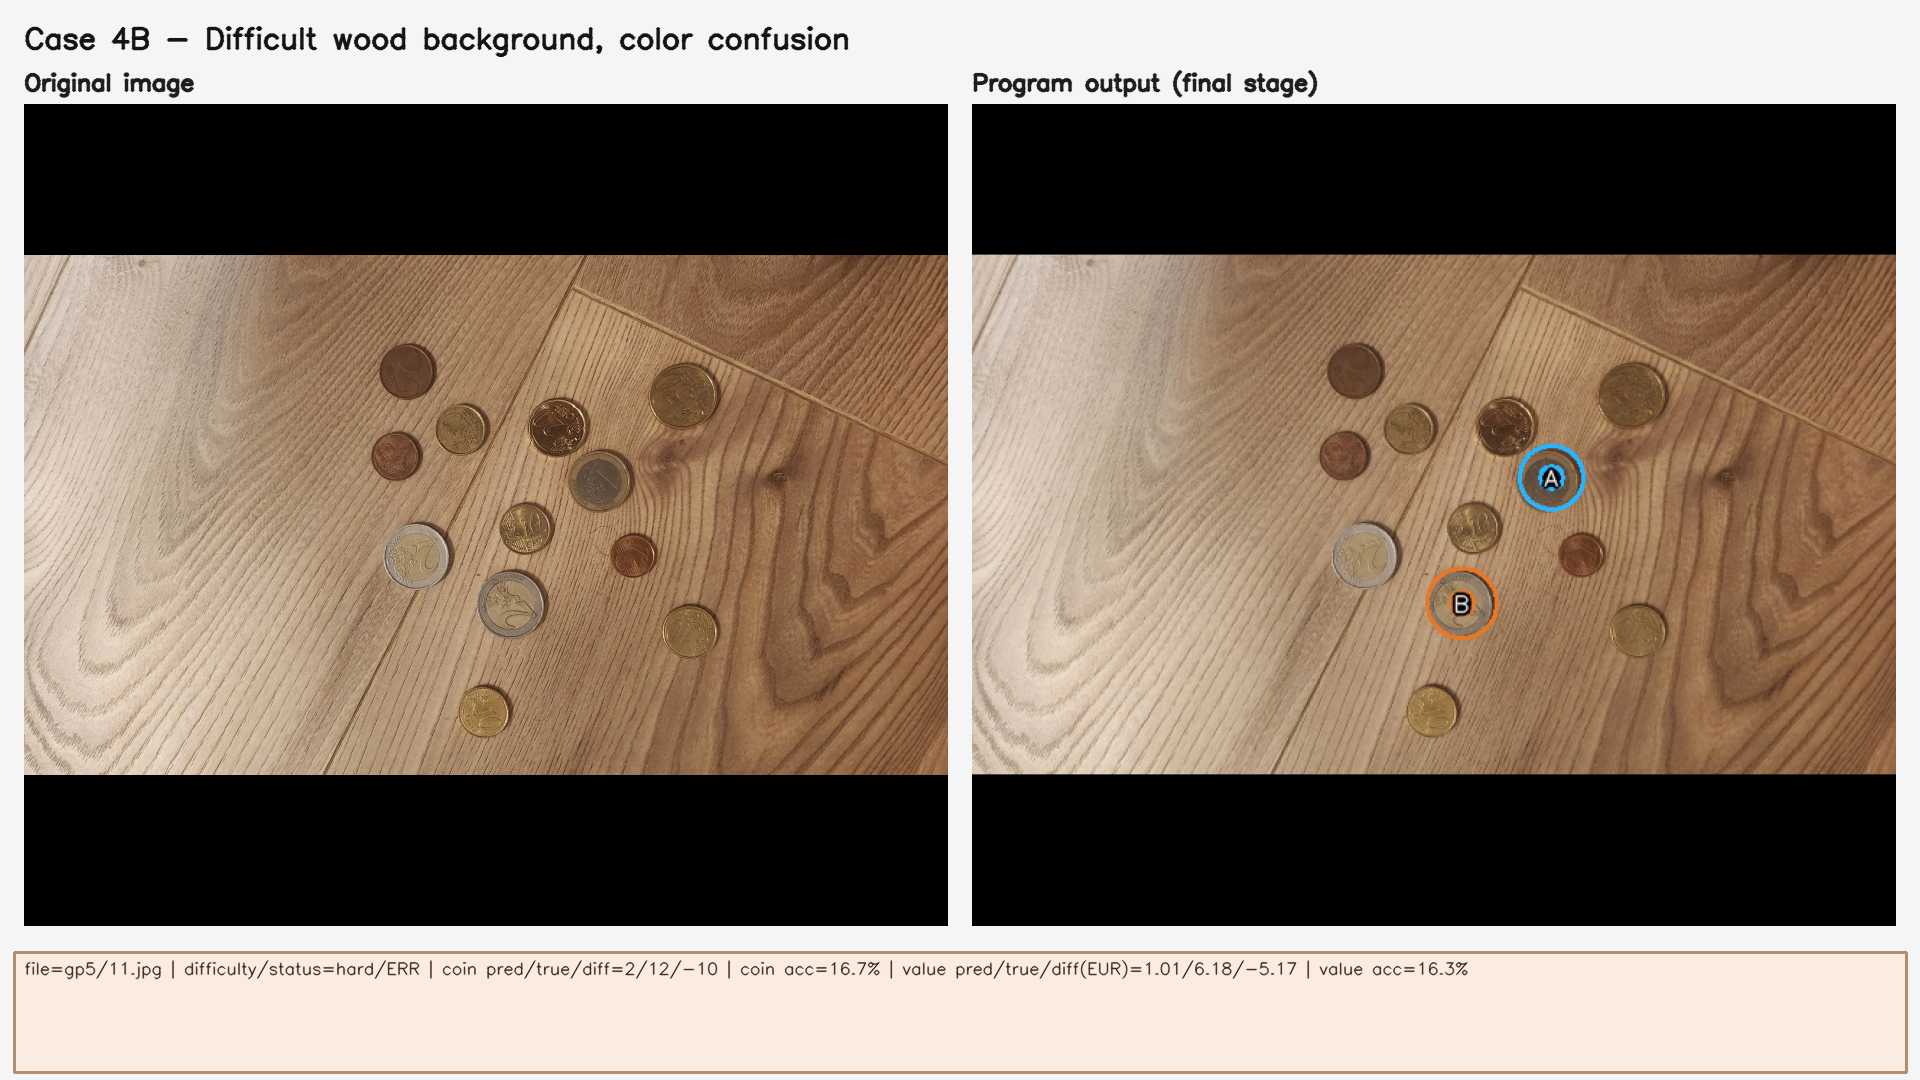
\includegraphics[width=0.985\linewidth,height=0.82\textheight,keepaspectratio]{panel_gp5_11.png}
\end{frame}

\begin{frame}{Case 4C: Hard Mixed Scene Near Coin Palette (gp5/13.jpg)}
  \centering
  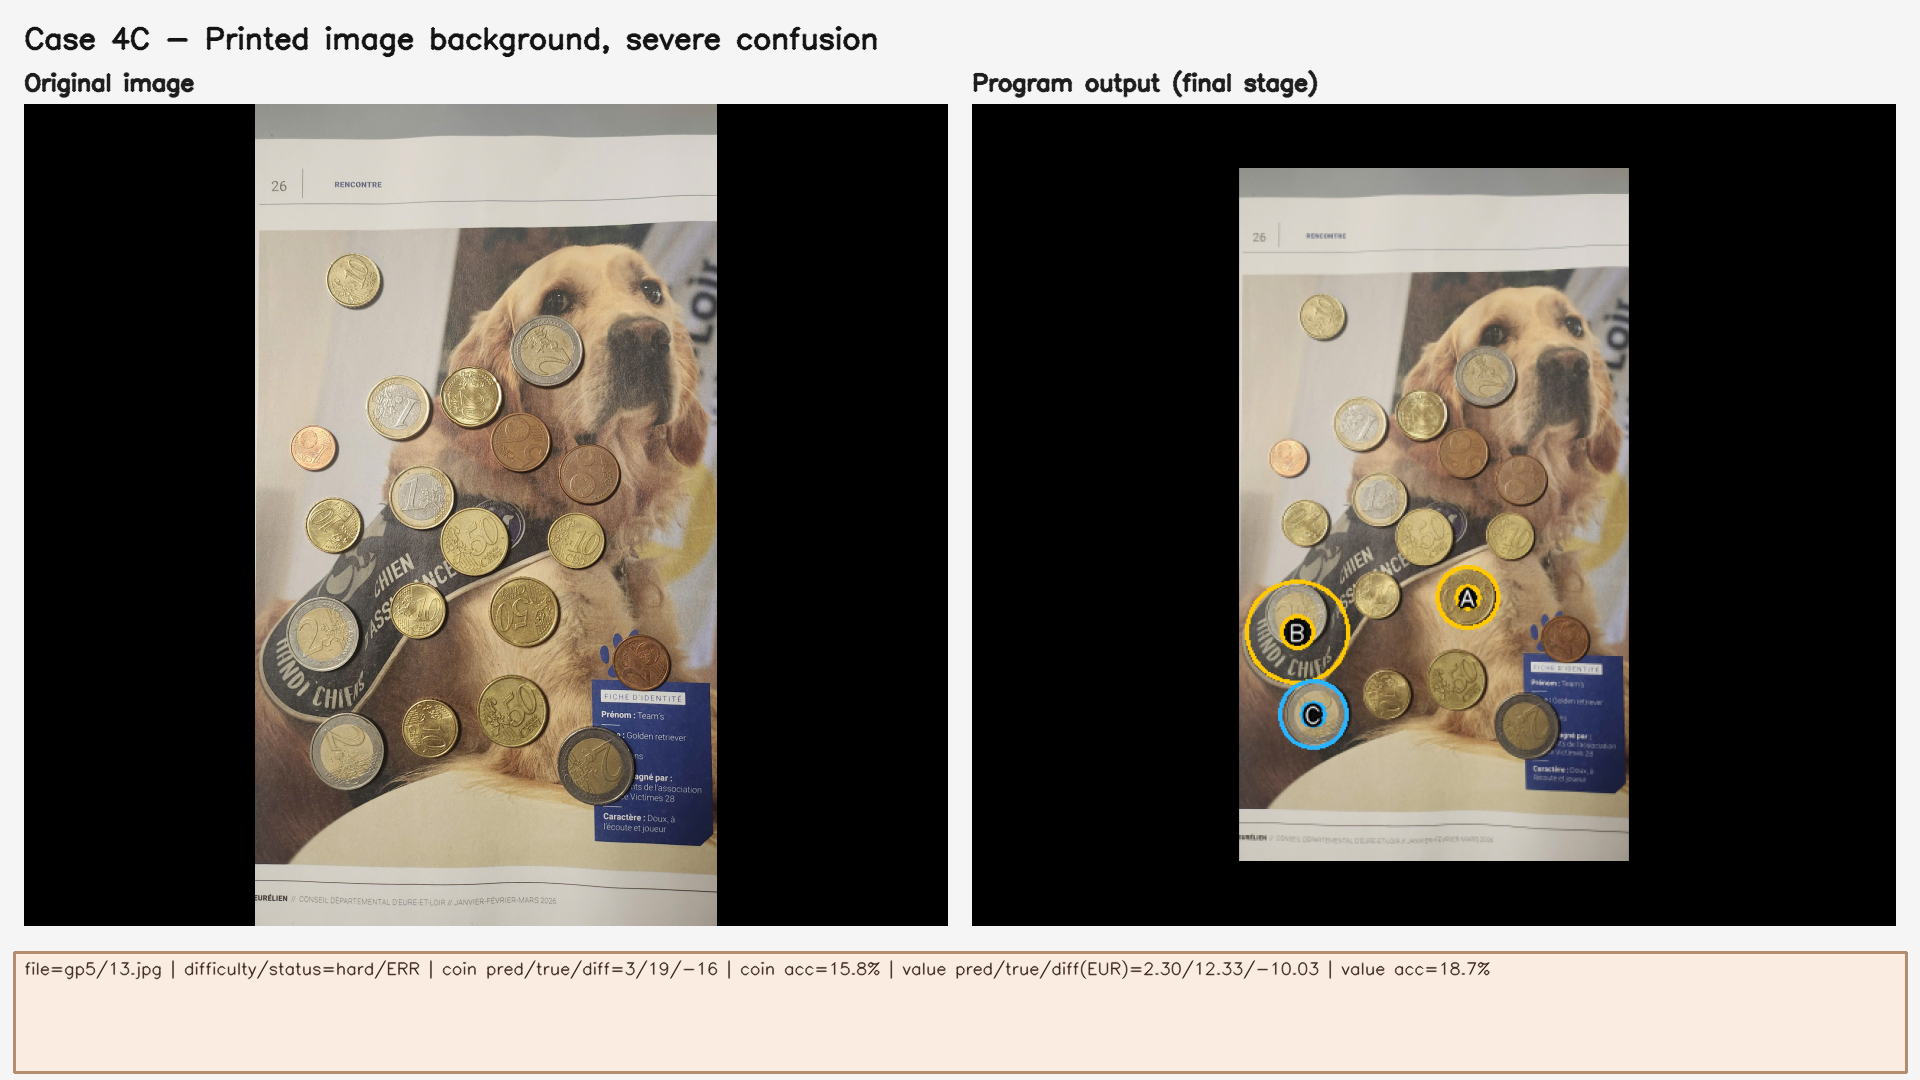
\includegraphics[width=0.985\linewidth,height=0.82\textheight,keepaspectratio]{panel_gp5_13.png}
\end{frame}

\begin{frame}{Case 4D: Very Hard Background (gp5/16.jpg)}
  \centering
  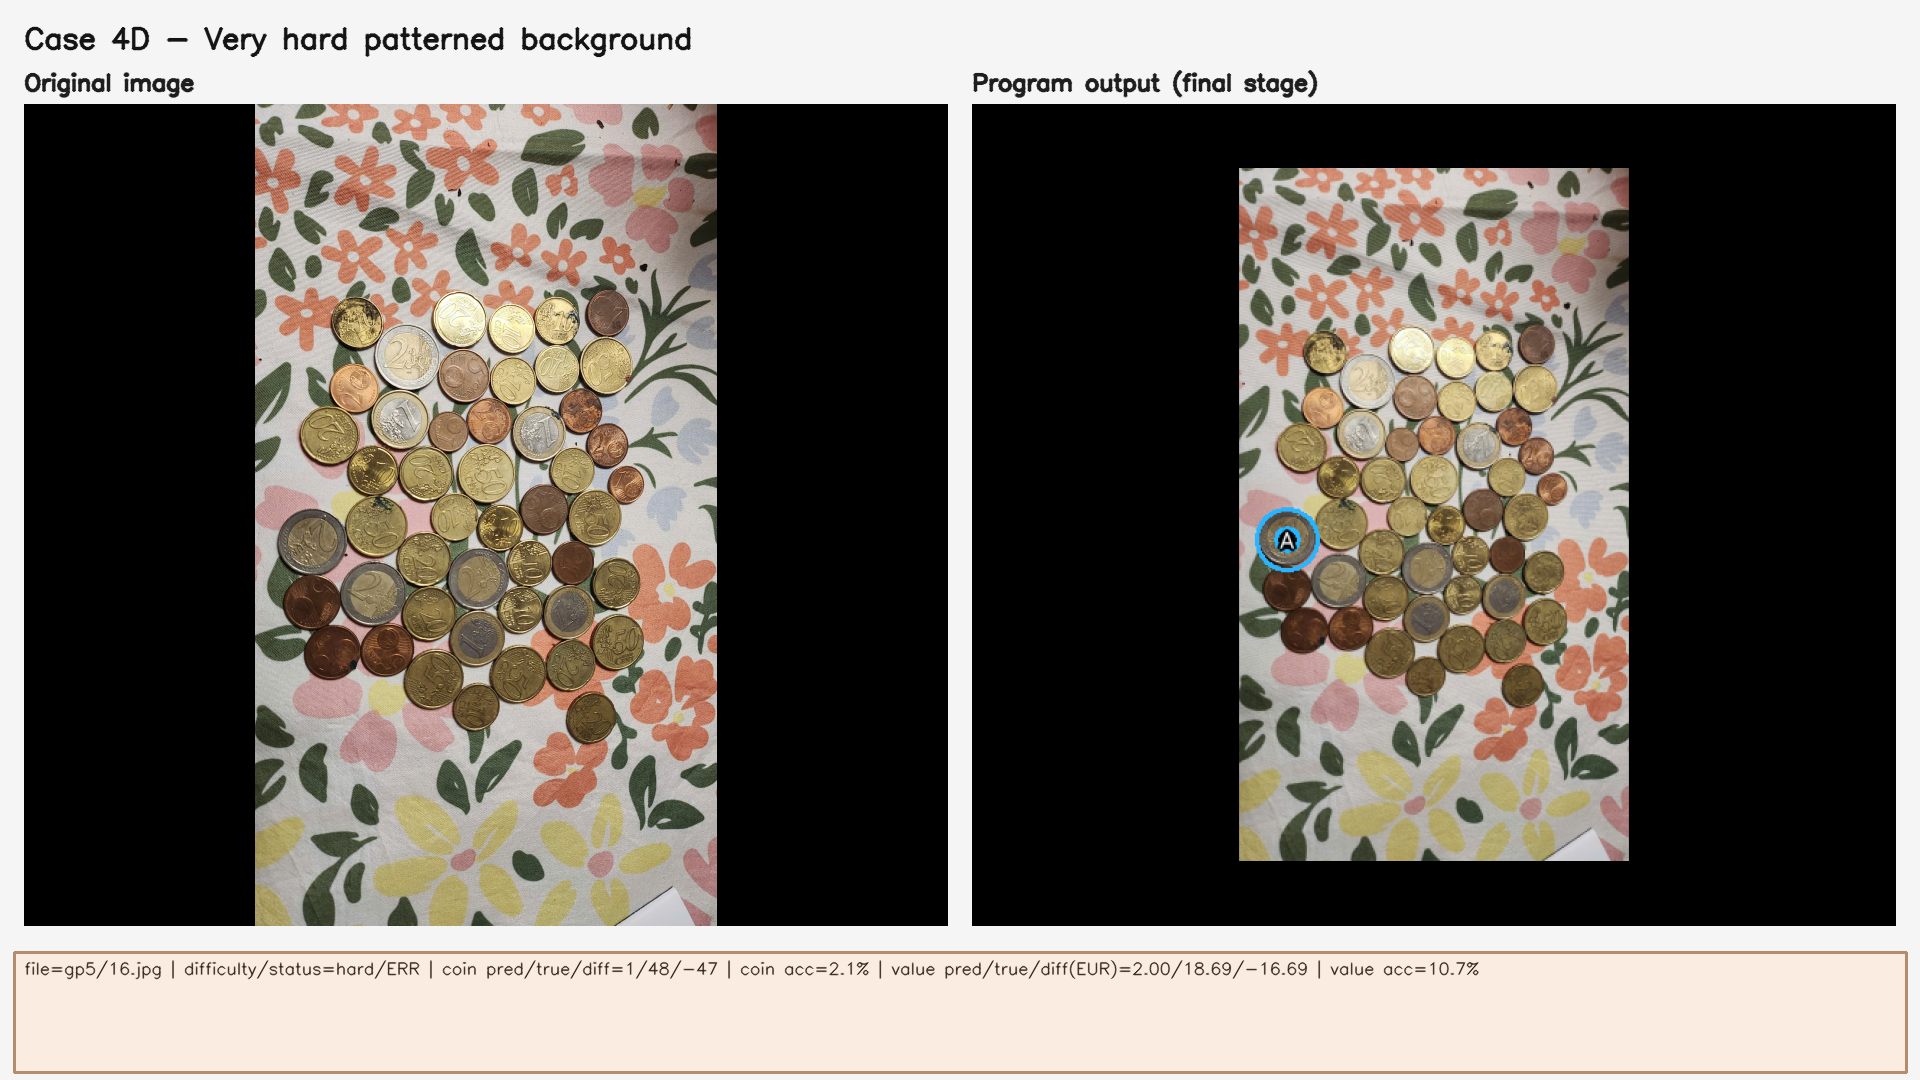
\includegraphics[width=0.985\linewidth,height=0.82\textheight,keepaspectratio]{panel_gp5_16.png}
\end{frame}

\begin{frame}{Case 5: Coins Too Close to Each Other}
  \centering
  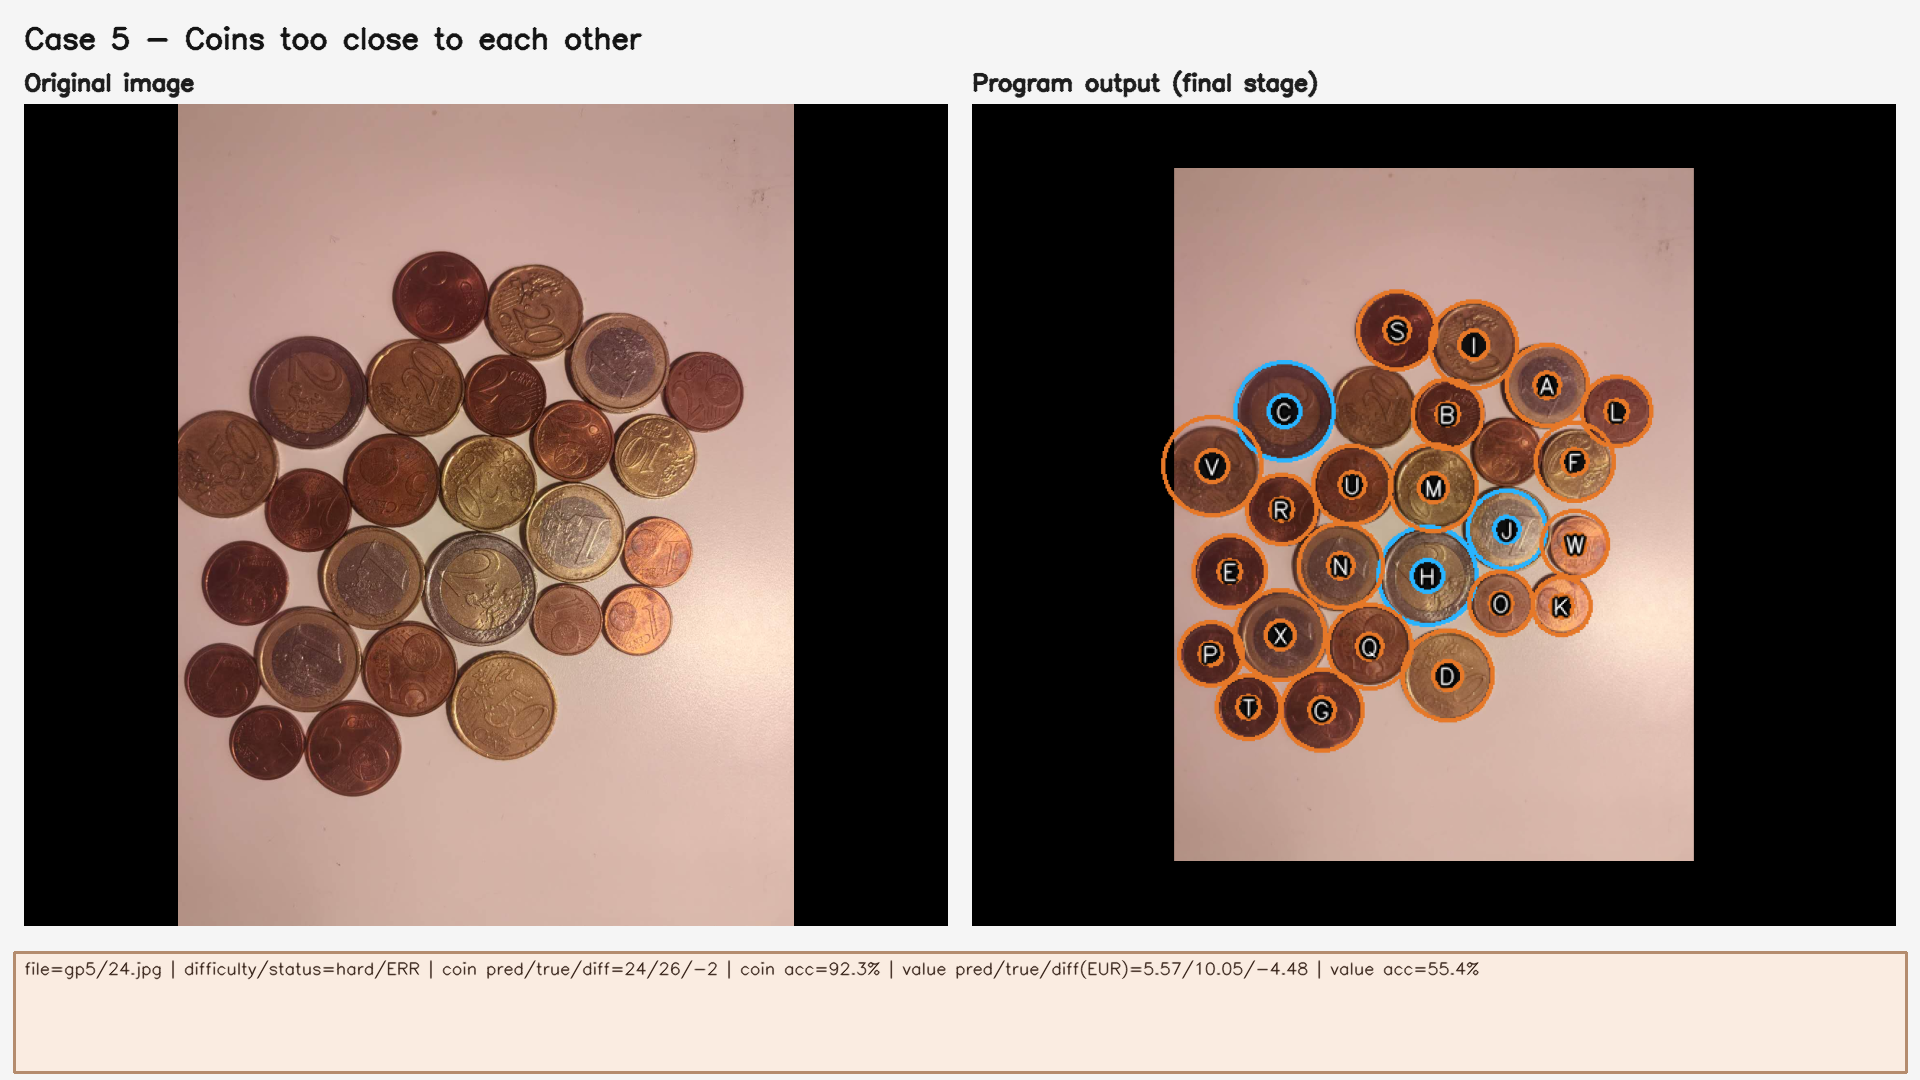
\includegraphics[width=0.985\linewidth,height=0.82\textheight,keepaspectratio]{panel_gp5_24.png}
\end{frame}

\begin{frame}{Case 6 (Assumed): Circle-like Background Noise + Color Confusion}
  \centering
  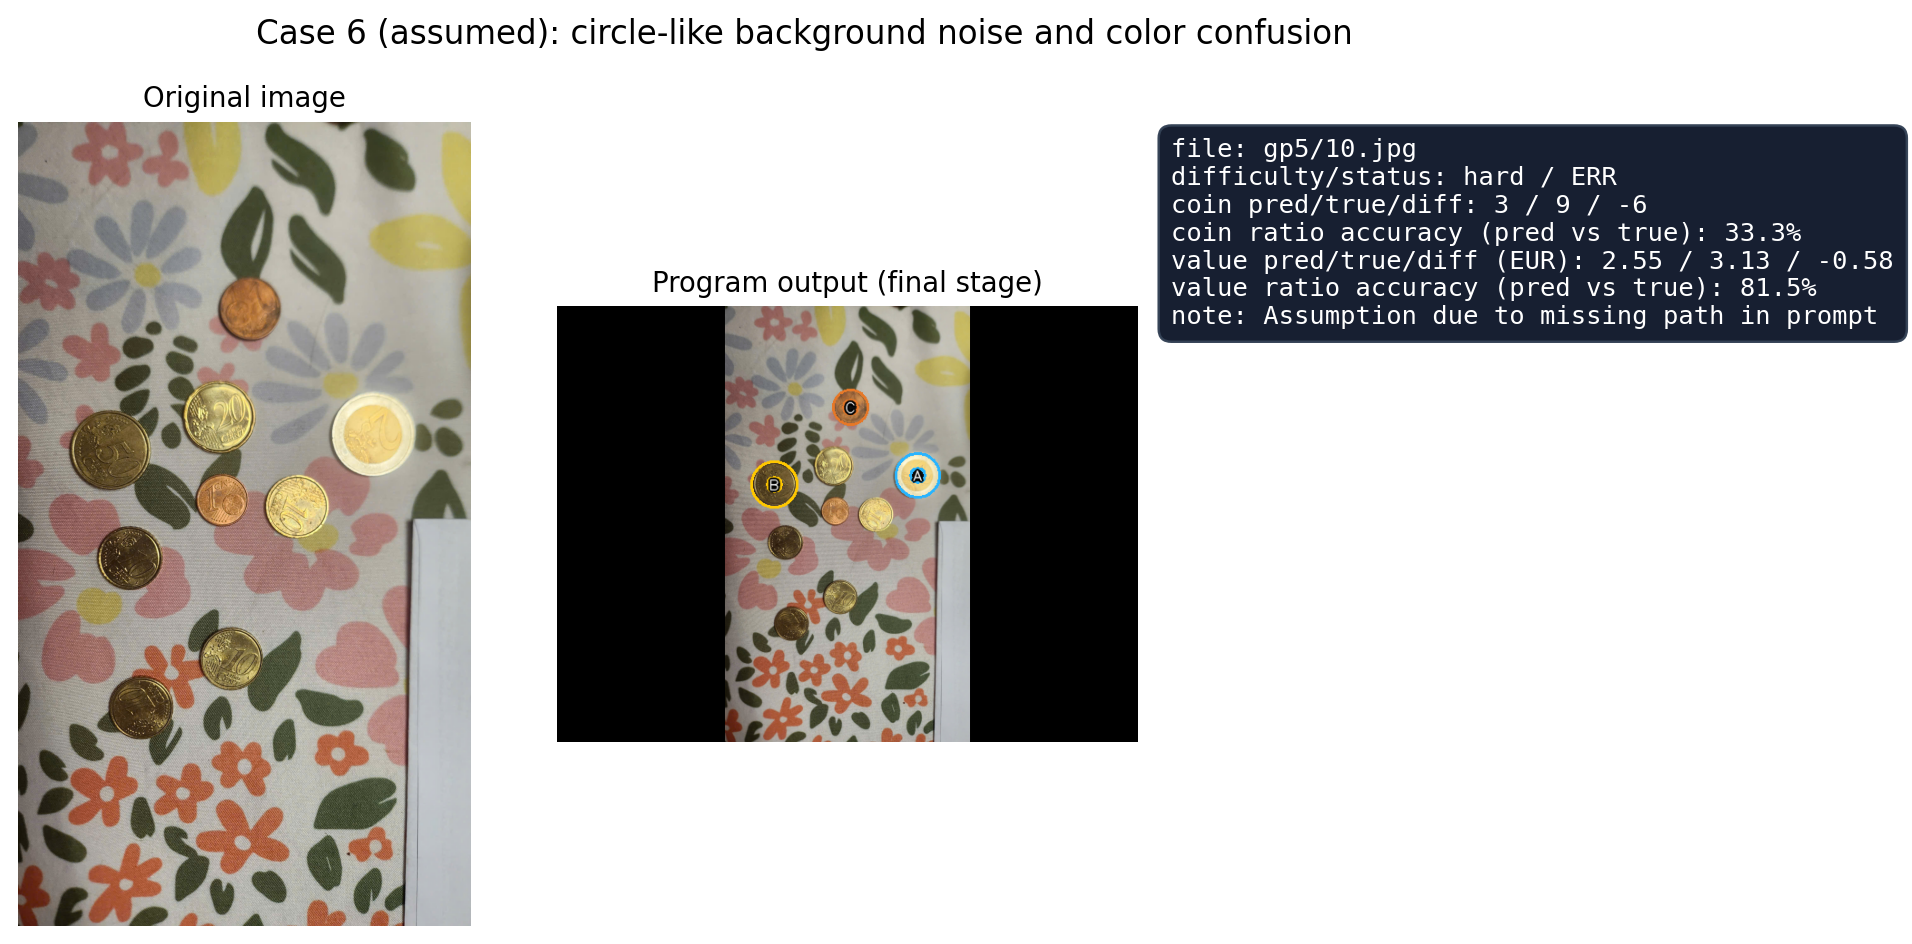
\includegraphics[width=0.985\linewidth,height=0.82\textheight,keepaspectratio]{case_gp5_10_assumed_item6.png}
\end{frame}

\begin{frame}{Failure Case: gp5/17.jpg (45$^\circ$ Camera Angle + Clutter)}
  \centering
  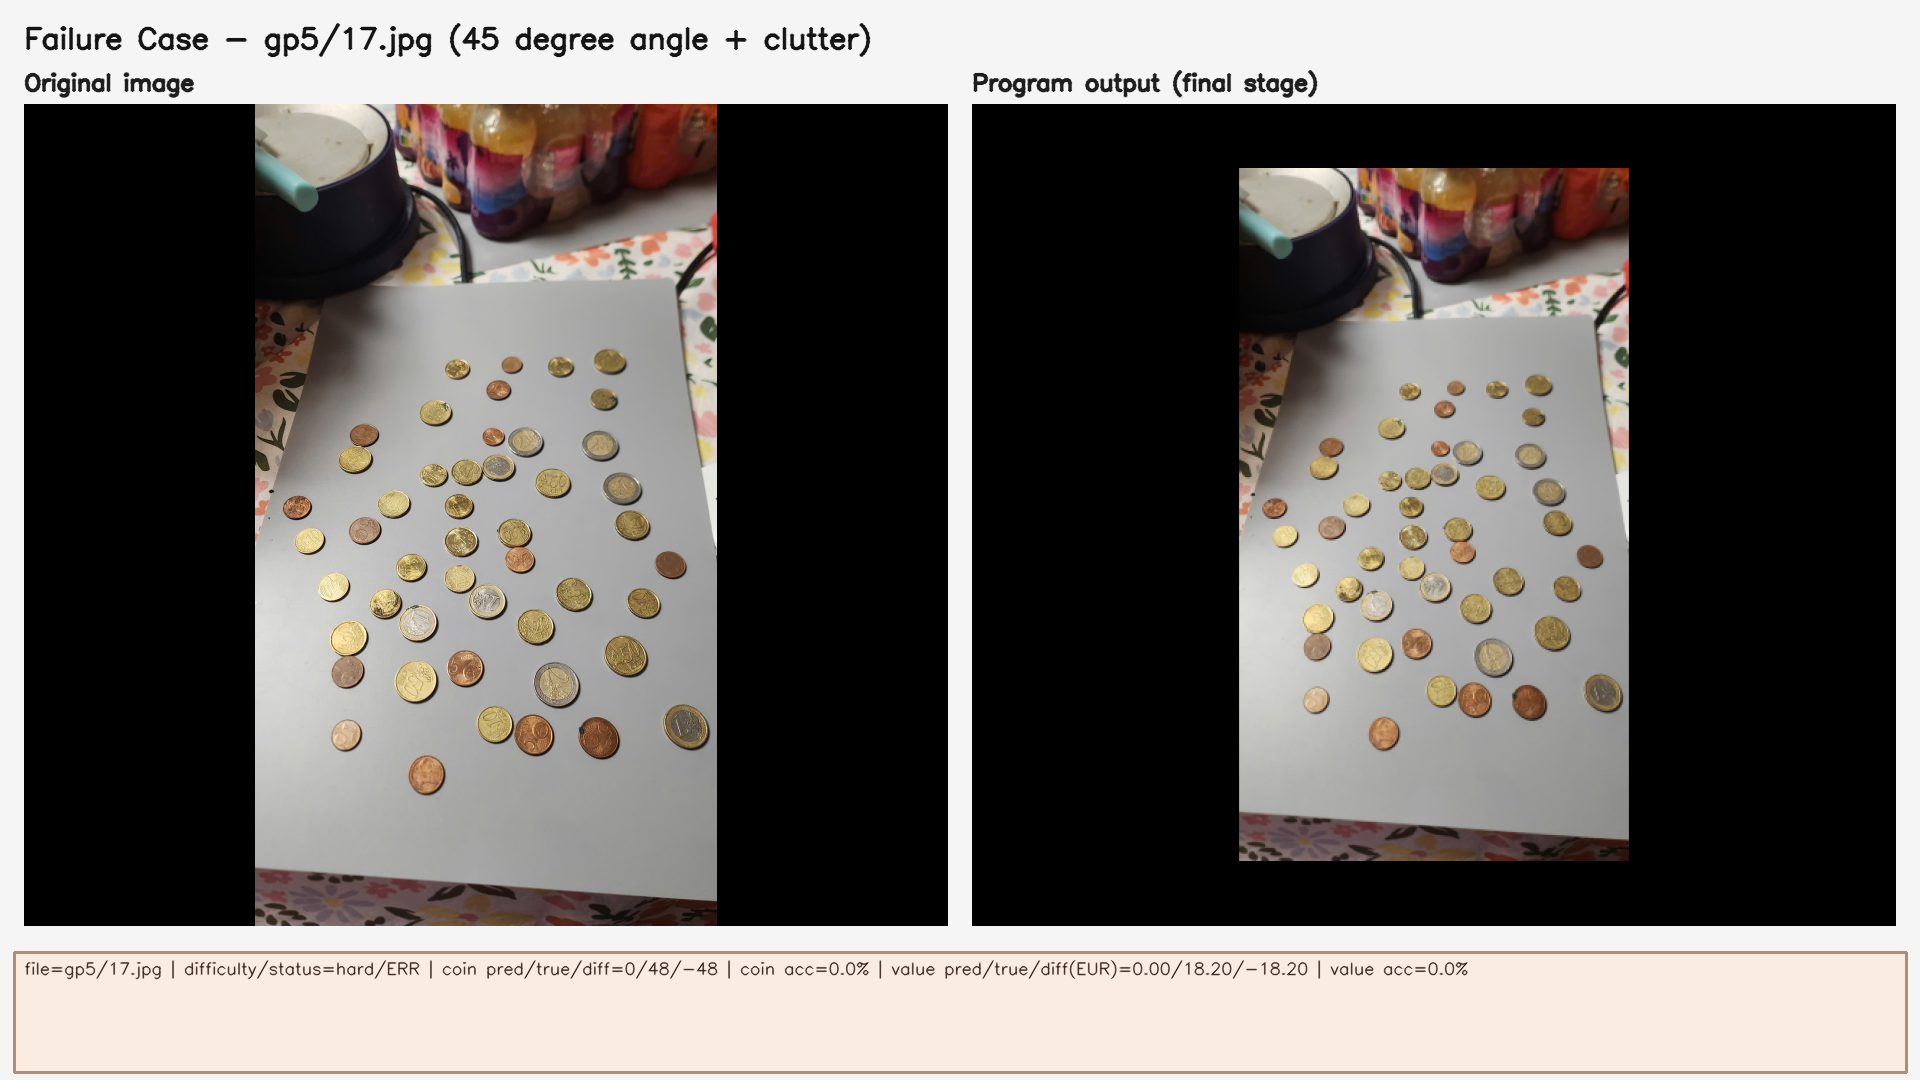
\includegraphics[width=0.985\linewidth,height=0.82\textheight,keepaspectratio]{panel_gp5_17_fail.png}
\end{frame}

\begin{frame}{Failure Case: gp3/3\_9.jpg (Dense Layout + Hard Background)}
  \centering
  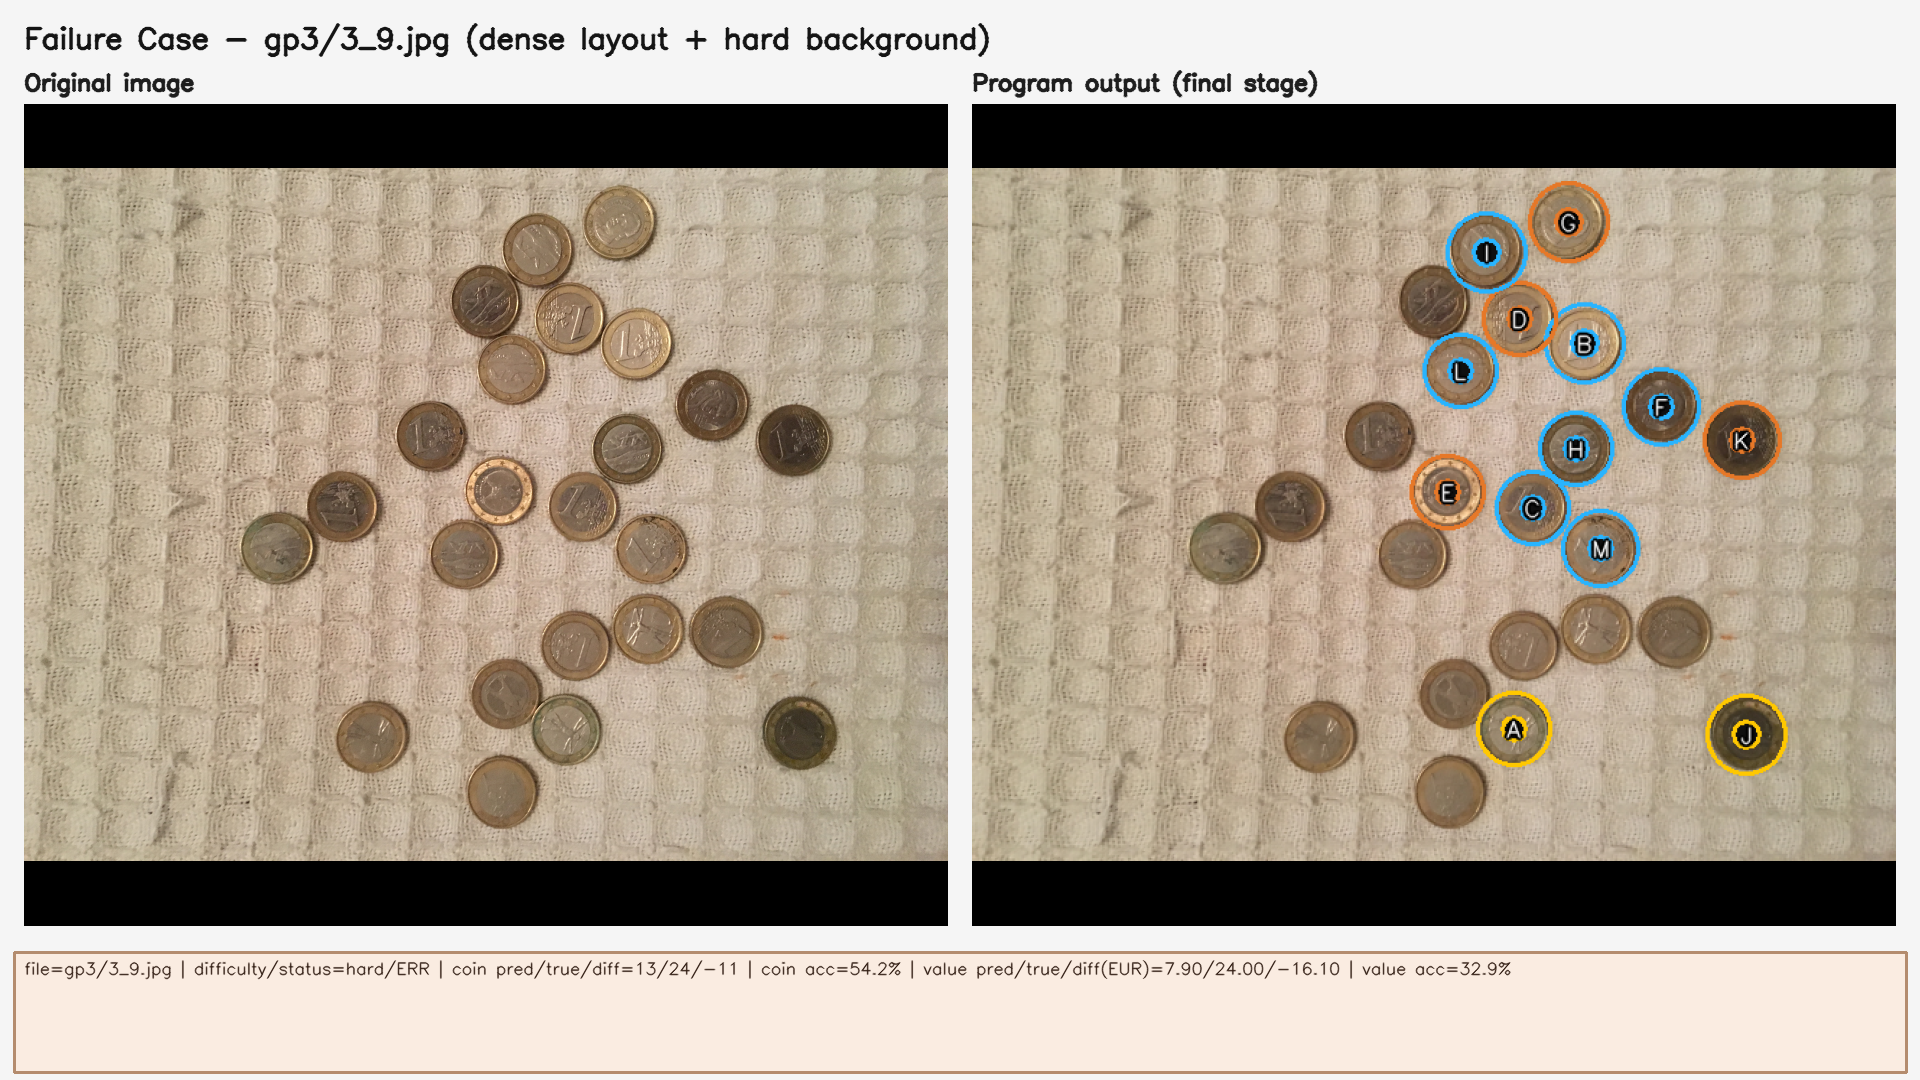
\includegraphics[width=0.985\linewidth,height=0.82\textheight,keepaspectratio]{panel_gp3_3_9_fail.png}
\end{frame}

\begin{frame}{Normal/Easy Example: gp2/1.jpeg}
  \centering
  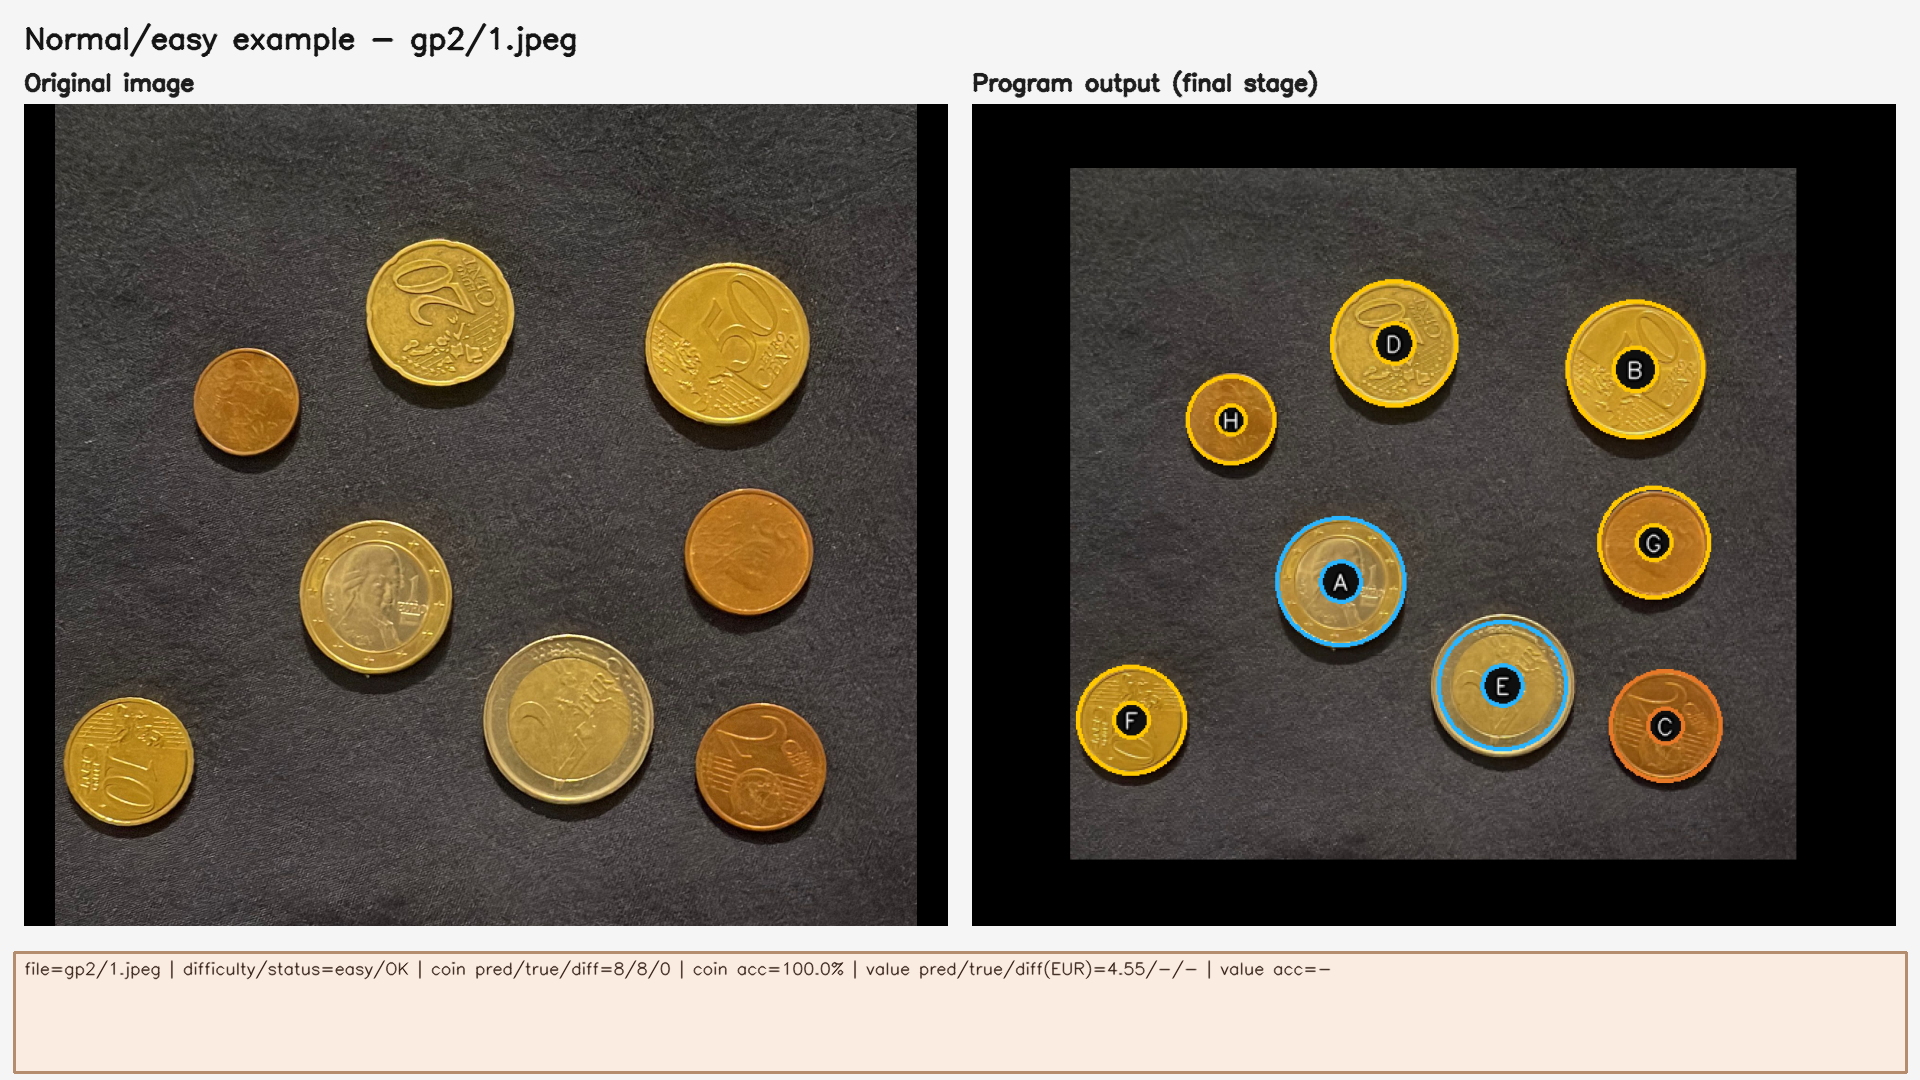
\includegraphics[width=0.985\linewidth,height=0.82\textheight,keepaspectratio]{panel_gp2_1_easy.png}
\end{frame}

\begin{frame}{Normal/Easy Example: gp2/4.jpeg}
  \centering
  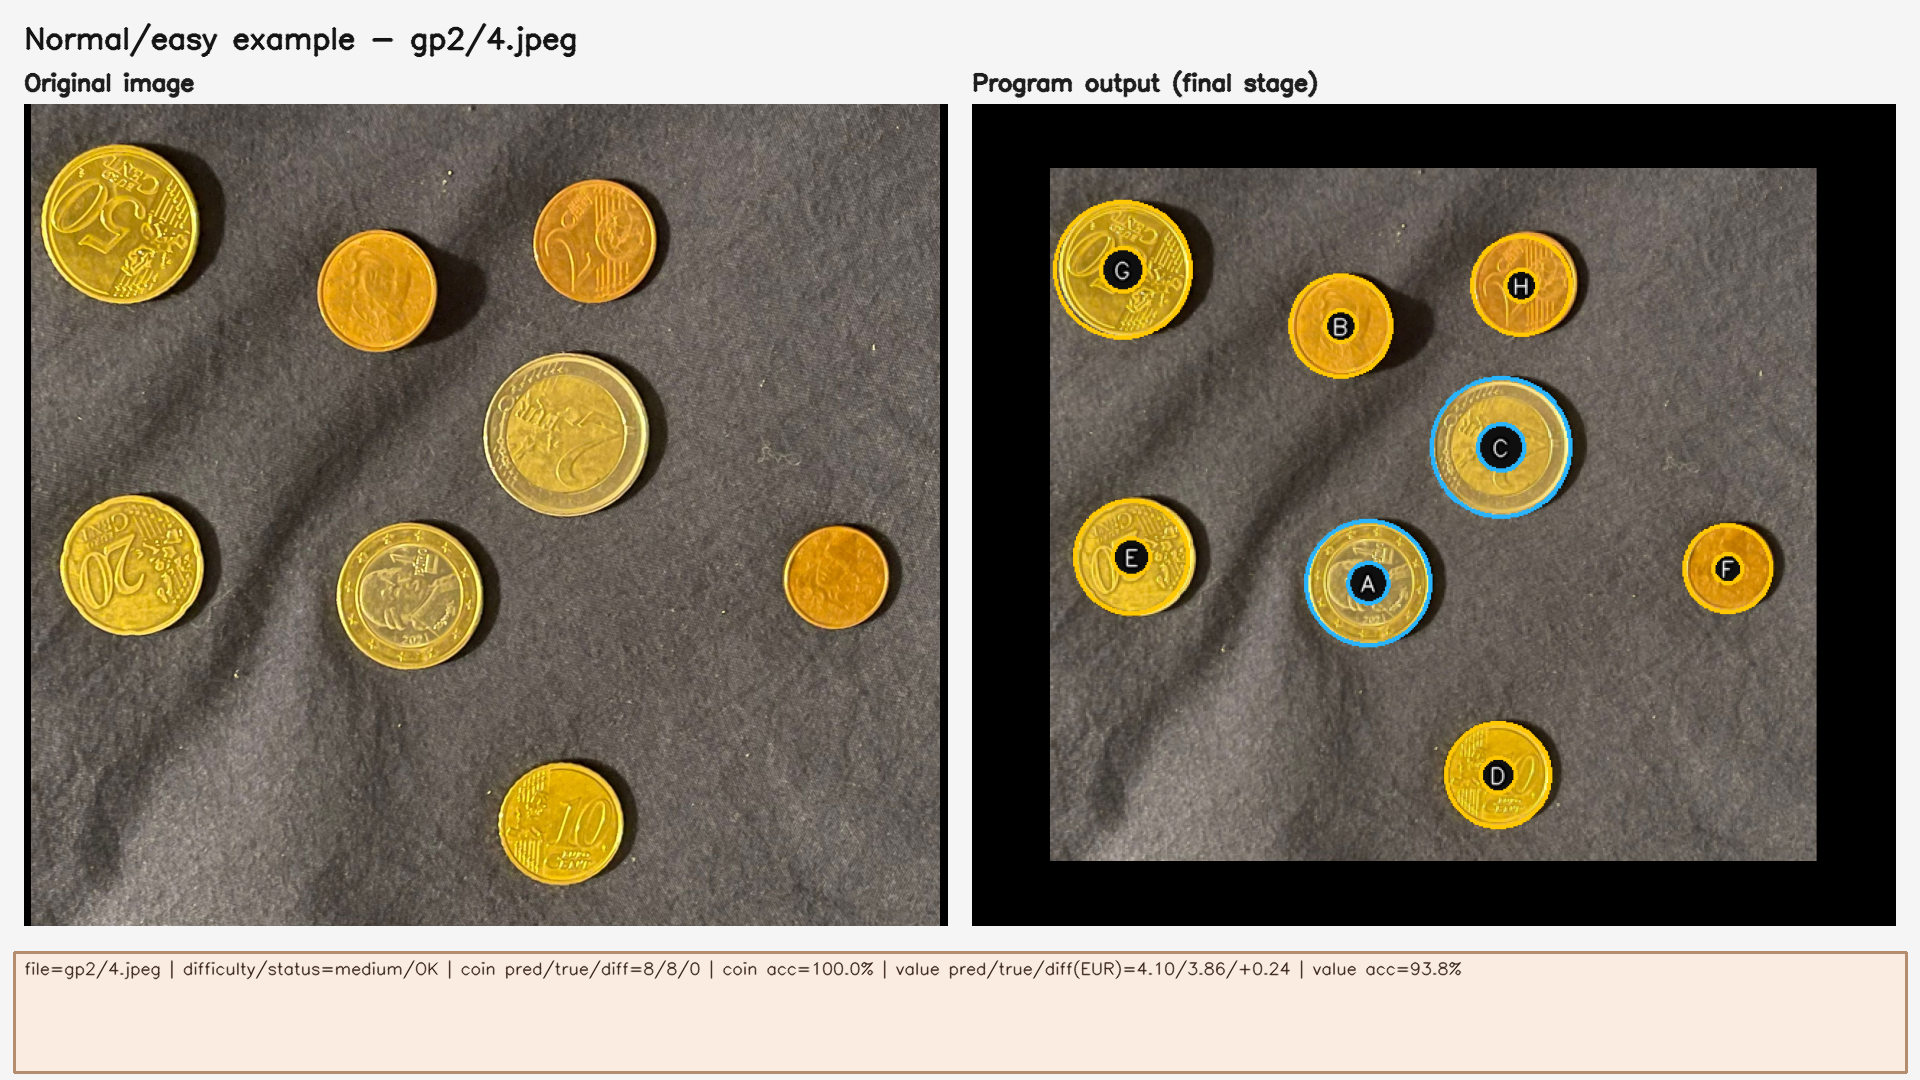
\includegraphics[width=0.985\linewidth,height=0.82\textheight,keepaspectratio]{panel_gp2_4_easy.png}
\end{frame}

\begin{frame}{Normal/Easy Example: gp8/IMG\_1143.png}
  \centering
  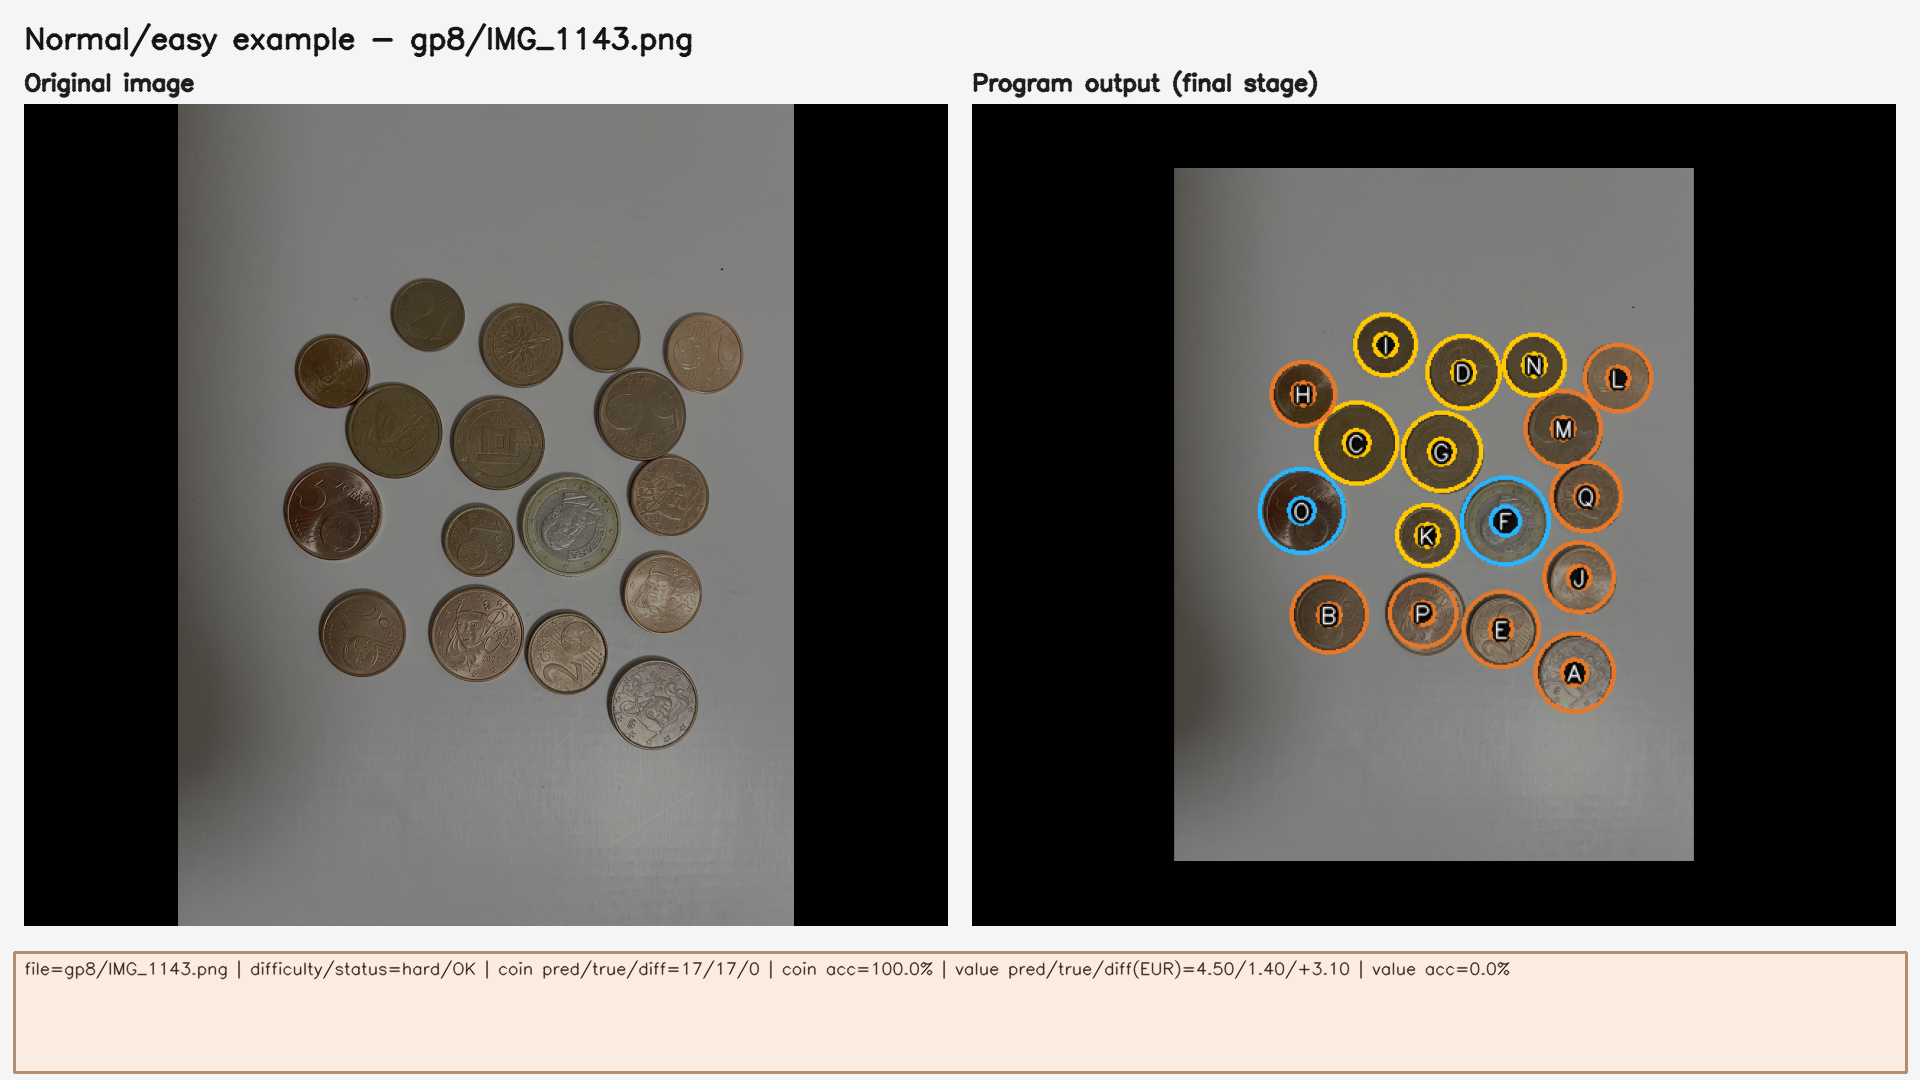
\includegraphics[width=0.985\linewidth,height=0.82\textheight,keepaspectratio]{panel_gp8_1143_easy.png}
\end{frame}

\section{Quantitative Results and Analysis}

\begin{frame}{Global Performance Snapshot}
  \begin{columns}[T]
    \begin{column}{0.56\textwidth}
      \centering
      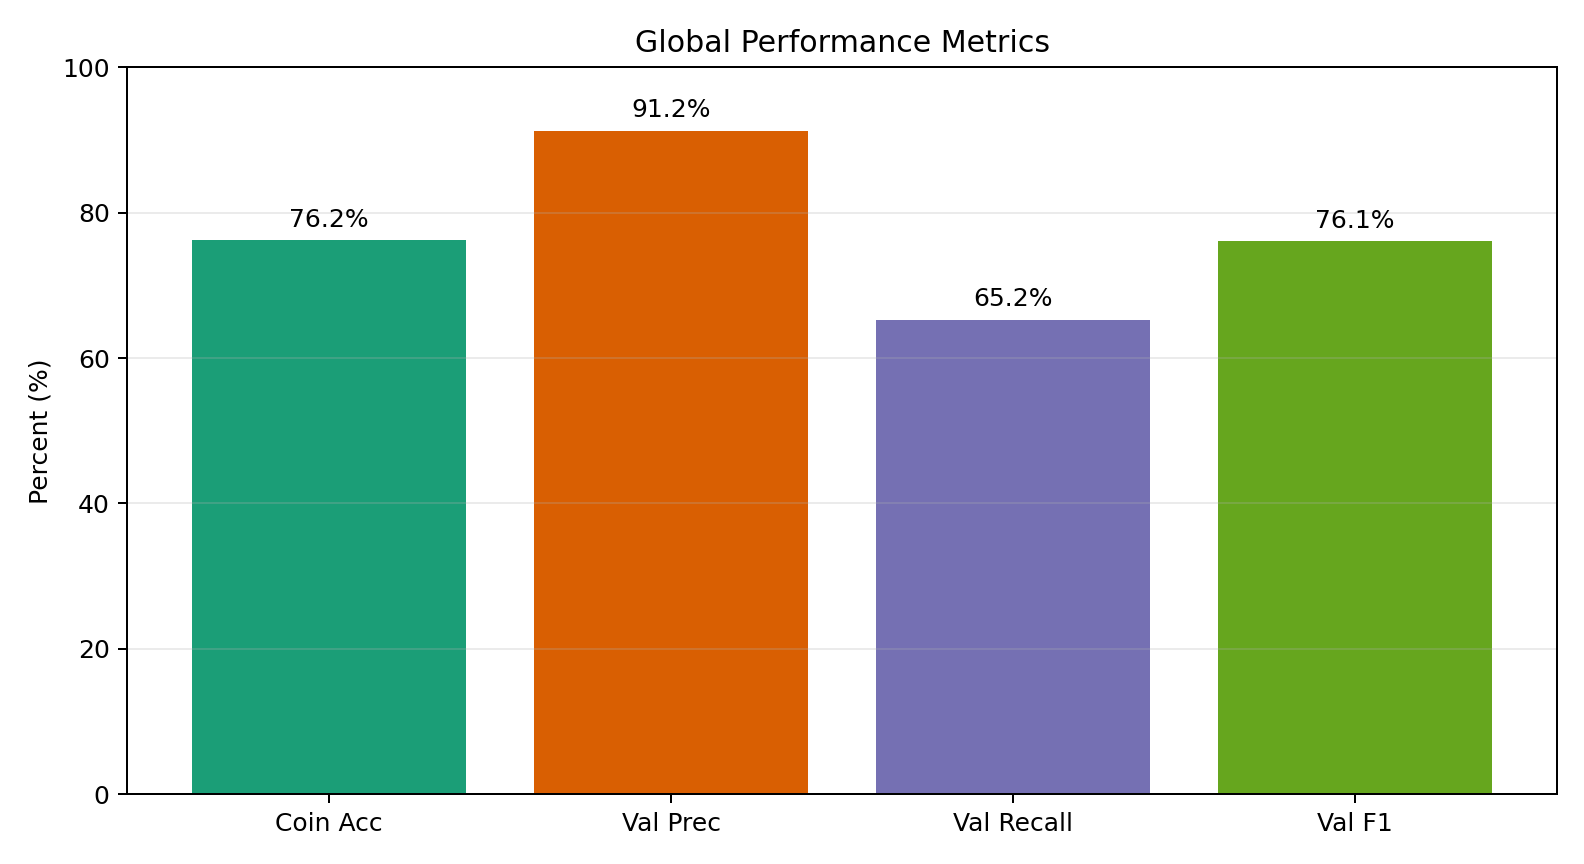
\includegraphics[width=\linewidth]{metrics_overview.png}
    \end{column}
    \begin{column}{0.44\textwidth}
      \small
      \textbf{Observed strengths}
      \begin{itemize}
        \item Strong performance on clean groups (\texttt{gp2}, \texttt{gp7}, \texttt{gp6}).
        \item Stable full-run completion: 106/106 images processed.
      \end{itemize}
      \textbf{Observed limits}
      \begin{itemize}
        \item Coin exact-match accuracy is 76.19\% overall.
        \item Hard groups (\texttt{gp3}, \texttt{gp5}) dominate large count/value errors.
        \item Value MAE rises sharply when many coins are missed in cluttered scenes.
      \end{itemize}
    \end{column}
  \end{columns}
\end{frame}

\begin{frame}{Difficulty Distribution and Error Landscape}
  \begin{columns}[T]
    \begin{column}{0.49\textwidth}
      \centering
      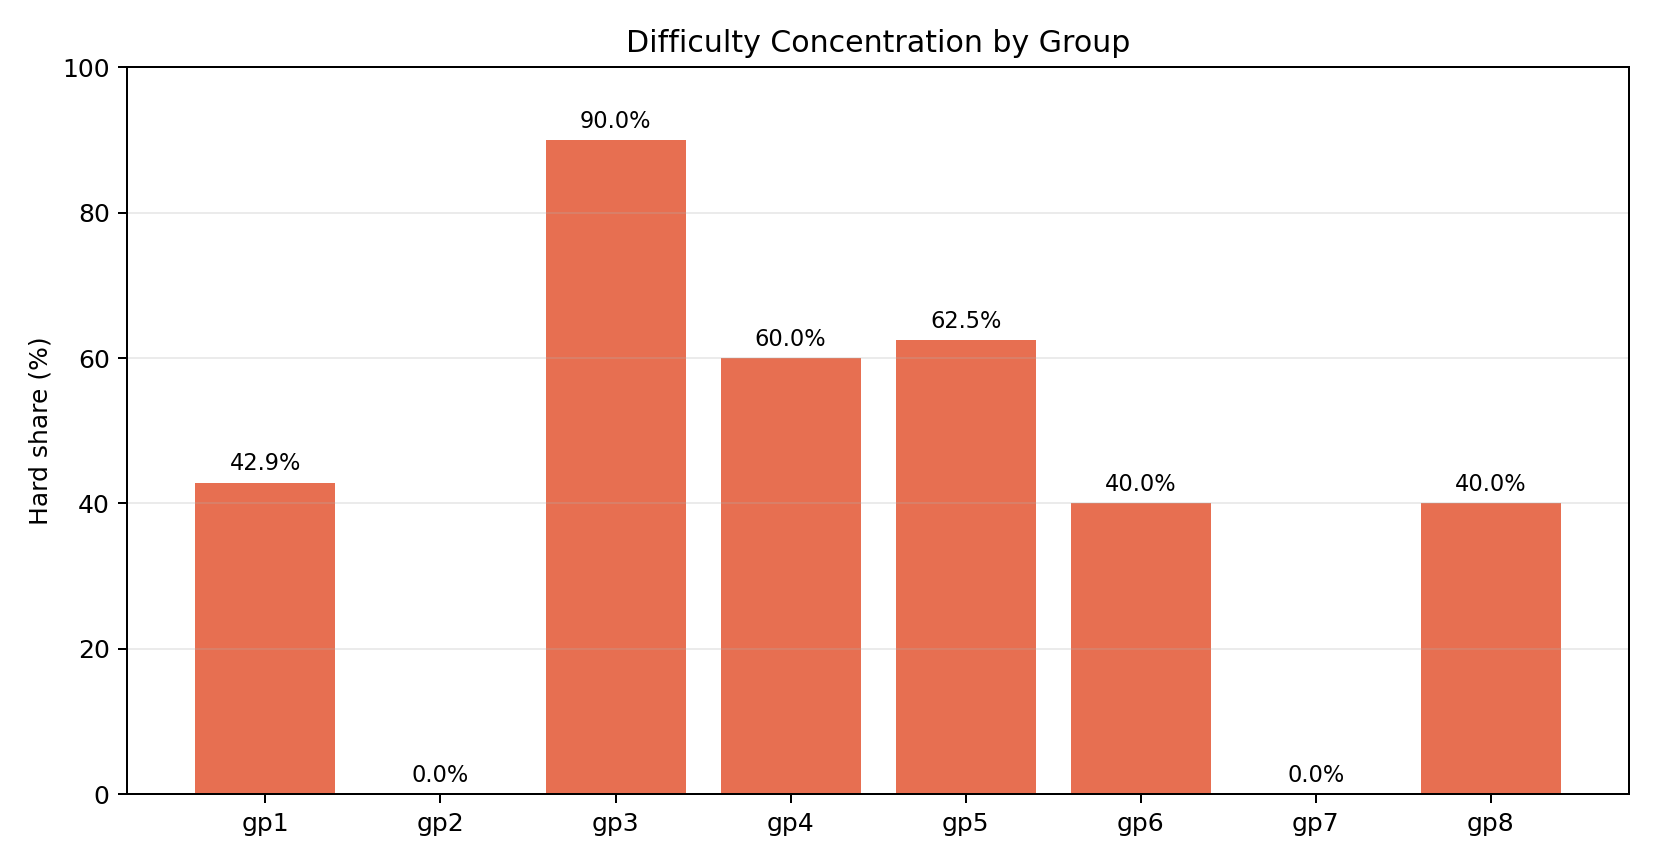
\includegraphics[width=\linewidth]{group_hard_share.png}
    \end{column}
    \begin{column}{0.49\textwidth}
      \centering
      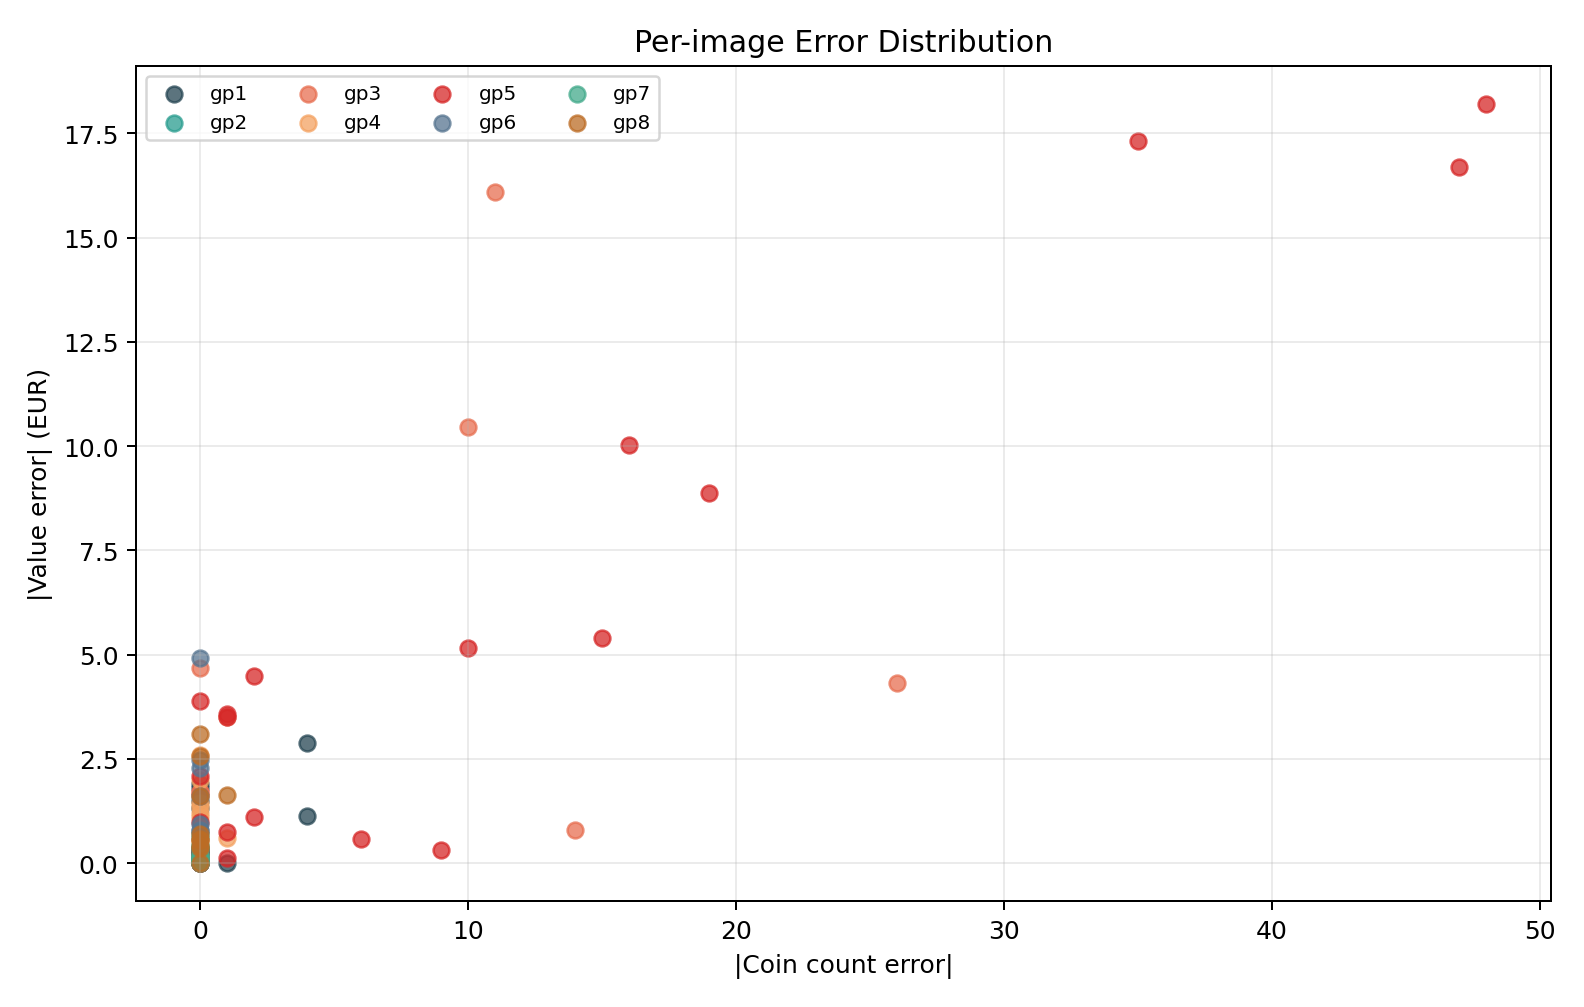
\includegraphics[width=\linewidth]{error_scatter.png}
    \end{column}
  \end{columns}

  \vspace{0.2em}
  \small
  \begin{itemize}
    \item Hard-share peaks in \texttt{gp3} and \texttt{gp5}, matching visual clutter/overlap.
    \item Scatter confirms correlation: large coin-count errors tend to create large value errors.
  \end{itemize}
\end{frame}

\begin{frame}{Interpretation of Requested Cases}
  \begin{itemize}
    \item \textbf{gp2/3.jpeg}: overlap is present, but boundary contrast is sufficient for correct count/value.
    \item \textbf{gp1/25.png}: coin spacing is good, but background texture/color biases value classification.
    \item \textbf{gp3/3\_10.jpg}: angle and reflections reduce radius consistency and count accuracy.
    \item \textbf{gp5/17.jpg}: full failure (\(0/48\)), with strong clutter and roughly \(45^\circ\) camera angle.
    \item \textbf{gp3/3\_9.jpg}: failure from dense layout + textured background causing merge/miss errors.
    \item \textbf{gp5 hard set}: colors/shapes in background overlap coin cues, causing severe misses.
    \item \textbf{gp5/24.jpg}: close packing causes near-touching circles and merge/split ambiguity.
  \end{itemize}
\end{frame}

\section{Conclusion}

\begin{frame}{What We Learned}
  \textbf{What worked}
  \begin{itemize}
    \item Modular pipeline with clear debug artifacts per stage.
    \item Adaptive Hough setup improved robustness over fixed parameters.
    \item Inner/border analysis provided useful color-family cues.
  \end{itemize}

  \textbf{Main failure modes}
  \begin{itemize}
    \item Strong texture/color similarity between coins and background (notably in \texttt{gp5}).
    \item Perspective angle and reflections changing apparent radius.
    \item Dense layouts and close coins causing circle separation ambiguity.
  \end{itemize}
\end{frame}

\begin{frame}{Next Steps}
  \begin{itemize}
    \item Add stronger segmentation before Hough (masking and region proposals).
    \item Improve overlap handling (multi-scale hypotheses + duplicate suppression).
    \item Add calibration with controlled reference objects.
    \item Explore learning-based detectors for hard groups while keeping explainability.
    \item Extend evaluation with per-denomination confusion analysis.
  \end{itemize}
\end{frame}

\begin{frame}
  \centering
  \Large Thank you
\end{frame}

\end{document}
